%%%%%%%%%%%%%%%%%%%%%%%%%%%%%%%%%%%%%%%%%%%%%%%%%%%%%%%%%%%%%%%%%%%%%%%%
%     LaTeX source code to approximate a NIST Technical report
%	  Instructions for authors: tinyurl.com/techpubsnist 
%	DOI watermark will be added on final PDF
% 	Developed by K. Miller, kmm5@nist.gov 
%	Last updated: 26-March-2019
%%%%%%%%%%%%%%%%%%%%%%%%%%%%%%%%%%%%%%%%%%%%%%%%%%%%%%%%%%%%%%%%%%%
\documentclass[12pt]{article}
\usepackage{adjustbox}
\usepackage{amsmath}
\usepackage{amsfonts}   % if you want the fonts
\usepackage{amssymb}    % if you want extra symbols
\usepackage{booktabs}
\usepackage{bm}
\usepackage{chemformula}
\usepackage{float}
%\usepackage{fourier}

\usepackage[hang,flushmargin,bottom]{footmisc} % footnote format
\usepackage{graphicx}   % need for figures
\usepackage{mathptmx}
\usepackage{multicol}
\usepackage{physics}
\usepackage{rotating}
\usepackage{secdot}
\usepackage{siunitx} % Formats the units and values
\usepackage{tabulary}
\usepackage{textgreek}
\usepackage{textcomp}
\usepackage{tikz}
\usepackage[newparttoc]{titlesec}
\usepackage[utf8]{inputenc}
\usepackage{xcolor}
\usepackage{footmisc}
\titleformat{\section}{\normalsize\bfseries}{\thesection.}{1em}{}	% required for heading numbering style
\titleformat*{\subsection}{\normalsize\bfseries}

\usepackage{tocloft}	% change typeset, titles, and format list of appendices/figures/tables
\renewcommand{\cftdot}{}	
\renewcommand{\contentsname}{Table of Contents}
\renewcommand{\cftpartleader}{\cftdotfill{\cftdotsep}} % for parts
\renewcommand{\cftsecleader}{\cftdotfill{\cftdotsep}}
\renewcommand\cftbeforesecskip{\setlength{4pt}{}}
\addtolength{\cftfignumwidth}{1em}
\renewcommand{\cftfigpresnum}{\figurename\ }
\addtolength{\cfttabnumwidth}{1em}
\renewcommand{\cfttabpresnum}{\tablename\ }
\setlength{\cfttabindent}{0in}    %% adjust as you like
\setlength{\cftfigindent}{0in} 

\usepackage{enumitem}         % to control spacing between bullets/numbered lists

\usepackage[numbers,sort&compress]{natbib} % format bibliography 
\renewcommand{\bibsection}{}
\setlength{\bibsep}{0.0pt}

\usepackage[hidelinks]{hyperref}
\hypersetup{
	colorlinks = true,
urlcolor ={blue},
citecolor = {.},
linkcolor = {.},
anchorcolor = {.},
filecolor = {.},
menucolor = {.},
runcolor = {.}
pdftitle={},%%put title here to auto-fill properties of the PDF
pdfsubject={},%%put abstract here
pdfauthor={}, %%put author list here
pdfkeywords={} %%put keywords here
}
\urlstyle{same}

\usepackage{epstopdf} % converting EPS figure files to PDF

\usepackage{fancyhdr, lastpage}	% formatting document, calculating number of pages, formatting headers
\setlength{\topmargin}{-0.5in}
\setlength{\headheight}{39pt}
\setlength{\oddsidemargin}{0.25in}
\setlength{\evensidemargin}{0.25in}
\setlength{\textwidth}{6.0in}
\setlength{\textheight}{8.5in}

\usepackage{caption} % required for Figure labels
\captionsetup{font=small,labelfont=bf,figurename=Fig.,labelsep=period,justification=raggedright} 

%%%%%%%%%%% !!!!!! REQUIRED - FILL OUT METADATA HERE !!!!!!!! %%%%%%%%%%%%%%
%  	Report Number - fill in Report Number sent to you (see info below)
%   DOI Statement - fill in DOI sent to you 
%   Month Year - fill in Month and Year of Publication
%%%%%%%%%%%%%%%%%%%%%%%%%%%%%%%%%%%%%%%%%%%%%%%%%%%%%%%%%%%%%%%%%%%%%%%%%%%%%%%%%%%%%%
\newcommand{\pubnumber}{XXXX}
\newcommand{\DOI}{https://doi.org/10.6028/NIST.TN.XXXX}
\newcommand{\monthyear}{August 2019}


\newcommand*\chem[1]{\ensuremath{\mathrm{#1}}}

\newcommand\numberthis{\addtocounter{equation}{1}\tag{\theequation}}

%%%%%%%%%%%%%%%%%%%%%%%%%%%%%%%%%%%%%%%%%%%%%%%%%%%%%%%%%%%%%%%%%%%%
%   	BEGIN DOCUMENT 
%%%%%%%%%%%%%%%%%%%%%%%%%%%%%%%%%%%%%%%%%%%%%%%%%%%%%%%%%%%%%%%%%%%%
\begin{document}
	\urlstyle{rm} % Format style of \url   
	
%%%%%%%%%%%%%%%%%%%%%%%%%%%%%%%%%%%%%%%%%%%%%%%%%%%%%%%%%%%%%%%%%%%%
%   Cover Page is REQUIRED and must contain the information 
%	displayed here, at a minimum. Additional artwork may be included 
%	(e.g., official project/conference logo, etc.).
%	Pub Number automated based on metadata
%%%%%%%%%%%%%%%%%%%%%%%%%%%%%%%%%%%%%%%%%%%%%%%%%%%%%%%%%%%%%%%%%%%%
	\begin{titlepage}
		\begin{flushright}
%%%%%%%%%%%%%%%%%%%%%%%%%%%%%%%%%%%%%%%%%%%%%%%%%%%%%%%%%%%%%%%%%%%%
% 	Automated based on metadata - delete if not applicable
%%%%%%%%%%%%%%%%%%%%%%%%%%%%%%%%%%%%%%%%%%%%%%%%%%%%%%%%%%%%%%%%%%%%
\LARGE{\textbf{NIST Technical Note \pubnumber}}\\
\vfill
%%%%%%%%%%%%%%%%%%%%%%%%%%%%%%%%%%%%%%%%%%%%%%%%%%%%%%%%%%%%%%%%%%%%
%	Title 
%%%%%%%%%%%%%%%%%%%%%%%%%%%%%%%%%%%%%%%%%%%%%%%%%%%%%%%%%%%%%%%%%%%%
\Huge{\textbf{The Structure of Medium-Scale Pool Fires}}\\
\vfill
%%%%%%%%%%%%%%%%%%%%%%%%%%%%%%%%%%%%%%%%%%%%%%%%%%%%%%%%%%%%%%%%%%%%
%	Authors - add complete list of authors, affiliations will be 
%   added on title page
%%%%%%%%%%%%%%%%%%%%%%%%%%%%%%%%%%%%%%%%%%%%%%%%%%%%%%%%%%%%%%%%%%%%
\large Ryan Falkesntein-Smith\\
\large Anthony Hamins\\
\large Kunhyuk Sung\\
\large Jian Chen\\
\vfill
%%%%%%%%%%%%%%%%%%%%%%%%%%%%%%%%%%%%%%%%%%%%%%%%%%%%%%%%%%%%%%%%%%%%
%	The DOI is automated based on metadata.	
%%%%%%%%%%%%%%%%%%%%%%%%%%%%%%%%%%%%%%%%%%%%%%%%%%%%%%%%%%%%%%%%%%%%
\normalsize This publication is available free of charge from:\\
\DOI\\
\vfill
%%%%%%%%%%%%%%%%%%%%%%%%%%%%%%%%%%%%%%%%%%%%%%%%%%%%%%%%%%%%%%%%%%%%
%	NIST LOGO - keep as-is
%%%%%%%%%%%%%%%%%%%%%%%%%%%%%%%%%%%%%%%%%%%%%%%%%%%%%%%%%%%%%%%%%%%%


\includegraphics[width=0.3\linewidth]{NIST-logo}\\ 


\end{flushright}
\end{titlepage}
\begin{titlepage}
%%%%%%%%%%%%%%%%%%%%%%%%%%%%%%%%%%%%%%%%%%%%%%%%%%%%%%%%%%%%%%%%%%%%
%	Title Page is REQUIRED
%%%%%%%%%%%%%%%%%%%%%%%%%%%%%%%%%%%%%%%%%%%%%%%%%%%%%%%%%%%%%%%%%%%%
\begin{flushright}
%%%%%%%%%%%%%%%%%%%%%%%%%%%%%%%%%%%%%%%%%%%%%%%%%%%%%%%%%%%%%%%%%%%%
%   Publication Series & Number - automated
%%%%%%%%%%%%%%%%%%%%%%%%%%%%%%%%%%%%%%%%%%%%%%%%%%%%%%%%%%%%%%%%%%%%
\LARGE{\textbf{NIST Technical Note \pubnumber}}\\
\vfill 
%%%%%%%%%%%%%%%%%%%%%%%%%%%%%%%%%%%%%%%%%%%%%%%%%%%%%%%%%%%%%%%%%%%%
%	Title 
%%%%%%%%%%%%%%%%%%%%%%%%%%%%%%%%%%%%%%%%%%%%%%%%%%%%%%%%%%%%%%%%%%%%
\Huge{\textbf{The Structure of Medium-Scale Pool Fires}}\\
\vfill
%%%%%%%%%%%%%%%%%%%%%%%%%%%%%%%%%%%%%%%%%%%%%%%%%%%%%%%%%%%%%%%%%%%%
%	Author Order and Grouping. Always identify the primary author/creator first (s/he does not have to be a NIST author). For publications with multiple authors, group authors by their organizational affiliation. The organizational groupings and the names within each grouping should generally be ordered by decreasing level of contribution.
%	For non-NIST authors, list their city and state below their organization name.
%	For NIST authors, include the Division and Laboratory names (but do not include their city and state).
%%%%%%%%%%%%%%%%%%%%%%%%%%%%%%%%%%%%%%%%%%%%%%%%%%%%%%%%%%%%%%%%%%%%
\normalsize Ryan Falkenstein-Smith\\
Anthony Hamins\\
Kunhyuk Sung\\
Jian Chen\\
\large
\textit{Fire Research Division}\\
\textit{Engineering Laboratory}\\
\vspace{12pt}
\vfill
%%%%%%%%%%%%%%%%%%%%%%%%%%%%%%%%%%%%%%%%%%%%%%%%%%%%%%%%%%%%%%%%%%%%
%   DOI Statement - automated
%%%%%%%%%%%%%%%%%%%%%%%%%%%%%%%%%%%%%%%%%%%%%%%%%%%%%%%%%%%%%%%%%%%%
\normalsize This publication is available free of charge from:\\
\DOI\\
\vfill
%%%%%%%%%%%%%%%%%%%%%%%%%%%%%%%%%%%%%%%%%%%%%%%%%%%%%%%%%%%%%%%%%%%%
%   Date - Month and Year - automated
%%%%%%%%%%%%%%%%%%%%%%%%%%%%%%%%%%%%%%%%%%%%%%%%%%%%%%%%%%%%%%%%%%%%
\normalsize \monthyear
\vfill
%%%%%%%%%%%%%%%%%%%%%%%%%%%%%%%%%%%%%%%%%%%%%%%%%%%%%%%%%%%%%%%%%%%%
%  Department of Commerce LOGO - leave as-is
%%%%%%%%%%%%%%%%%%%%%%%%%%%%%%%%%%%%%%%%%%%%%%%%%%%%%%%%%%%%%%%%%%%%	


\includegraphics[width=0.18\linewidth]{DoC-logo}\\ 
\vfill
%%%%%%%%%%%%%%%%%%%%%%%%%%%%%%%%%%%%%%%%%%%%%%%%%%%%%%%%%%%%%%%%%%%%
%  Department of Commerce & NIST Leadership 
%	will be updated as changes occur
%%%%%%%%%%%%%%%%%%%%%%%%%%%%%%%%%%%%%%%%%%%%%%%%%%%%%%%%%%%%%%%%%%%%
\footnotesize U.S. Department of Commerce\\
\textit{Wilbur L. Ross, Jr., Secretary}\\
\vspace{10pt}
National Institute of Standards and Technology\\
\textit{Walter Copan, NIST Director and Undersecretary of Commerce for Standards and Technology}
\end{flushright}
\end{titlepage}

\begin{titlepage}
%%%%%%%%%%%%%%%%%%%%%%%%%%%%%%%%%%%%%%%%%%%%%%%%%%%%%%%%%%%%%%%%%%%%
%   Disclaimer/CODEN page - required
%%%%%%%%%%%%%%%%%%%%%%%%%%%%%%%%%%%%%%%%%%%%%%%%%%%%%%%%%%%%%%%%%%%%
\begin{flushright}
\footnotesize  Certain commercial entities, equipment, or materials may be identified in this document in order to describe an experimental procedure or concept adequately. Such identification is not intended to imply recommendation or endorsement by the National Institute of Standards and Technology, nor is it intended to imply that the entities, materials, or equipment are necessarily the best available for the purpose.\\ 
\vfill
%%%%%%%%%%%%%%%%%%%%%%%%%%%%%%%%%%%%%%%%%%%%%%%%%%%%%%%%%%%%%%%%%%%%
%   This secton automated - do not change
%%%%%%%%%%%%%%%%%%%%%%%%%%%%%%%%%%%%%%%%%%%%%%%%%%%%%%%%%%%%%%%%%%%%
\normalsize \textbf{National Institute of Standards and Technology Technical Note \pubnumber\\ 
Natl. Inst. Stand. Technol. Tech. Note \pubnumber, \pageref{LastPage} pages (\monthyear)} \\
\textbf{CODEN: NTNOEF}\\
\vspace{12pt}
\textbf{This publication is available free of charge from: \DOI}
\vfill
\end{flushright}
\end{titlepage}
%%%%%%%%%%%%%%%%%%%%%%%%%%%%%%%%%%%%%%%%%%%%%%%%%%%%%%%%%%%%%%%%%%%%
%   Start front matter - page number starts with "i"
%%%%%%%%%%%%%%%%%%%%%%%%%%%%%%%%%%%%%%%%%%%%%%%%%%%%%%%%%%%%%%%%%%%%
\section*{Abstract}
This report documents a series of time-averaged local gas species measurements made throughout the centerline profile of moderate-sized methanol, ethanol, and acetone pool fires steadily burning in a quiescent environment. All gas species measurements are obtained using a Gas Chromatograph/ Mass Spectrometer system (GC/MSD). The volume fraction of each species was calculated via the number of moles identified by the GC/MSD at each location throughout the centerline profile of the fire. Soot mass fractions are simultaneously measured during the gas sampling process. The gas species volume and soot mass fractions were compared at different heights within the fire and across a variety of different fuels. Other fire parameters are measured as well, including time-averaged temperature measurements and mass burning rates. 
\section*{Keywords}
\normalsize Acetone fuel, Ethanol fuel, Gas species measurements. Methanol fuel, Moderate-sized pool fire\\
\pagebreak
%%%%%%%%%%%%%%%%%%%%%%%%%%%%%%%%%%%%%%%%%%%%%%%%%%%%%%%%%%%%%%%%%%%%
%   Table of Contents is required
% 	List of Tables & Figures required if more than 5 tables/figures
%%%%%%%%%%%%%%%%%%%%%%%%%%%%%%%%%%%%%%%%%%%%%%%%%%%%%%%%%%%%%%%%%%%%
\begin{center}
	\tableofcontents
	\listoftables
	\listoffigures
\end{center}
\pagebreak
%%%%%%%%%%%%%%%%%%%%%%%%%%%%%%%%%%%%%%%%%%%%%%%%%%%%%%%%%%%%%%%%%%%%
%   Start body of text - page number starts with "1"
%%%%%%%%%%%%%%%%%%%%%%%%%%%%%%%%%%%%%%%%%%%%%%%%%%%%%%%%%%%%%%%%%%%%
\section{Introduction}
\label{sec:intro}
Use of fire modeling, such as the Fire Dynamic Simulator (FDS)~\cite{FDS_Tech_Guide}, in fire protection engineering, has increased dramatically during the last decade due to the development of practical computational fluid dynamics fire models and the decreased cost of computational power. Today, fire protection engineers use models to design safer buildings, nuclear power plants, aircraft cabins, trains, and marine vessels, to name a few types of applications. To be reliable, the models require validation, which involves an extensive collection of experimental measurements. An objective of this report is to provide data for use in fire model evaluation by the research community.

A pool fire is a fundamental combustion configuration of interest in model development. In pool fires, the fuel surface is isothermal, flat and horizontal, providing a well-defined and straightforward setup for testing models and furthering the understanding of fire phenomena. In moderate and large-scale pool fires, radiative heat transfer is the dominant mechanism of heat feedback to the fuel surface. Species concentrations and temperatures have a significant influence on the radiative heat transfer. A zone of particular interest is the fuel rich-core between the flame and the pool surface, where gas species can absorb energy that would otherwise have been transferred to the fuel surface. Few studies in the literature studies have reported local chemical species measurements, which provide a deep understanding of the chemical structure of a pool fire and provide insight on critical kinetic, heat, and mass transfer processes.

The purpose of this study is to characterize the spatial distribution of stable gas-phase chemical species in moderate-scale liquid pool fires steadily burning in a well-ventilated quiescent environment. Here, methanol, ethanol, and acetone are the fuels of interest. Contrary to ethanol and acetone, fires established using methanol are unusual as no carbonaceous soot is present or emitted. These particular fuels are selected for research since the measurements complement results from previous studies, including analyses of the mass burning rate, the temperature and velocity fields, radiative emission, flame height, and pulsation frequency~\cite{Fisher1987,Hamins2016}. Additional characterization of this fire enables a more comprehensive understanding of its detailed structure, enhancing the understanding of fire physics.

\section{Description of Experiments}
\label{sec:Experiments}

The experimental setup used in this work to investigate pool fires has been documented previously~\cite{Hamins2016,Hamins1994,Hamins1991,Hamins1996,Lock2008}. Experiments are conducted under a canopy hood surrounded by a \SI{2.5}{m} x \SI{2.5}{m} x \SI{2.5}{m} enclosure made of a double-mesh screen wall. The walls of the enclosure were formed by a double layer of the wire-mesh screen (5 mesh/cm) to reduce the influence of compromising room flows that could disrupt the flow field. All measurements were made once the mass burning rate reached steady-state, achieved approximately \SI{10}{min} after ignition.

\subsection{Pool Burner Setup}
\label{ssec:Pool_Burner_Setup}
A circular, stainless-steel pan with an outer diameter of \SI{30}{cm}, a depth of \SI{15}{m}, and a wall thickness of \SI{0.16}{m} was used as the pool burner. As shown in Fig.~\ref{fig:Pool Burner}, the burner was placed within an overflow basin, which extended \SI{30}{cm} beyond the burner wall. The burner was fitted with legs such that the burner rim was positioned \SI{30}{m} above the ground. The bottom of the burner was maintained at a constant temperature by flowing water (\SI{20.0}{\degree C}~±~\SI{3.0}{\degree C}) through a \SI{3}{cm} section on the bottom of the fuel pan. Additionally, a fuel level indicator was positioned near the center of the burner to aid in maintaining the fuel level while burning.

\begin{figure}[h!]
	\centering
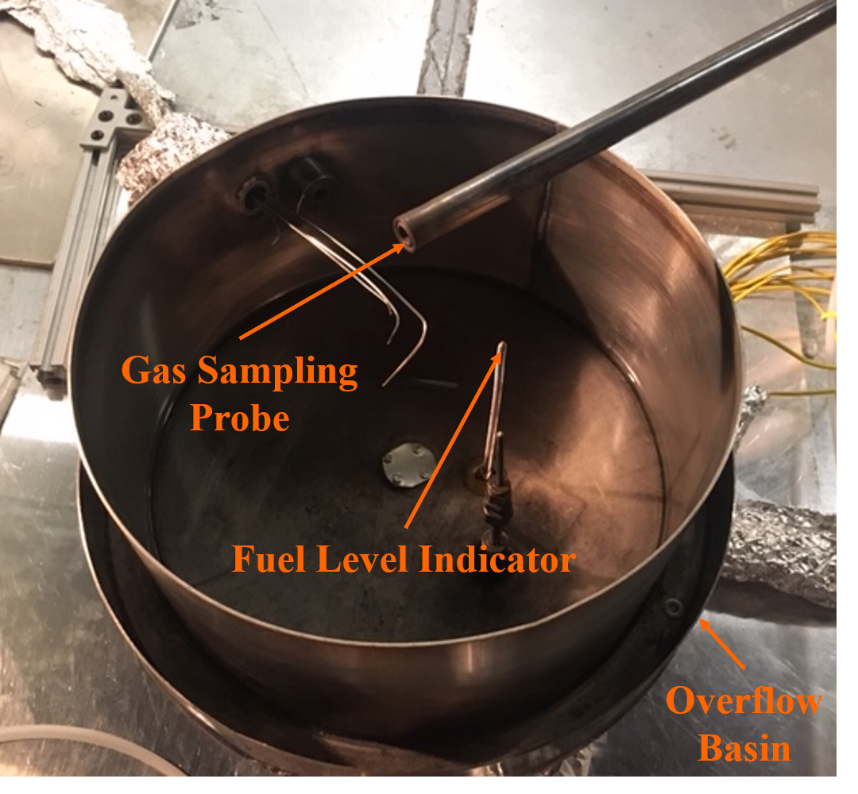
\includegraphics[width=10.0cm,keepaspectratio]{Pool_Burner.png}
	\caption[A \SI{30}{m} Pool Burner with fuel level indicator, overflow section, and quenching probe]{A \SI{30}{m} Pool Burner with fuel level indicator, overflow section, and quenching probe}
	\label{fig:Pool Burner}
\end{figure}

The time-averaged mass burning rate, $\dot{m}$, was determined from the rate at which fuel was delivered to the pool. Fuel to the burner was gravity fed from a reservoir positioned on a mass load cell located outside the enclosure and monitored by a data acquisition system (DAQ). As shown in Fig.~\ref{fig:Fuel_Level}, the fuel level was monitored via a fuel flow operator. The operator was able to observe a close up of a slightly discernible dimple (approximately \SI{2}{mm}) made from the fuel level indicator on the fuel surface using a live video feed. The fuel level was controlled by manually adjusting the fuel flow using a needle valve. The fuel level was set at \SI{10}{mm} below the burner rim to match previous experimental conditions \cite{Fisher1987,Hamins2016,Kim2019,Weckman1996}

\begin{figure}[h!]
	\centering
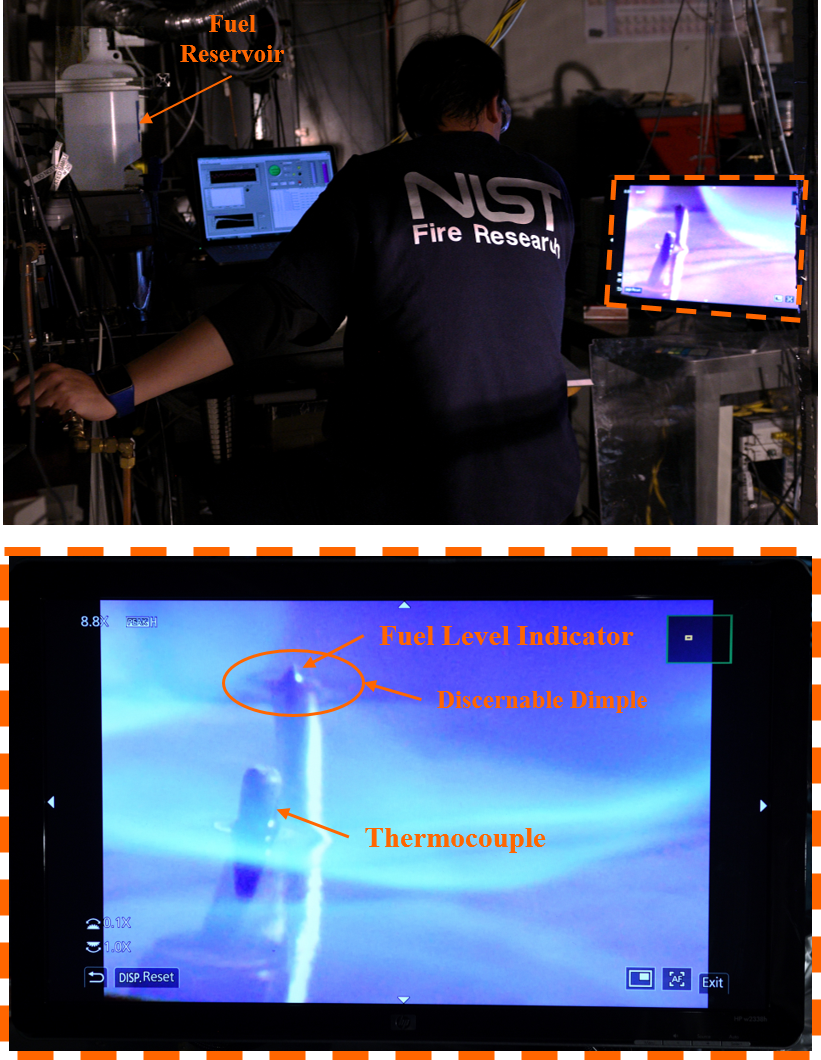
\includegraphics[width=14.0cm,keepaspectratio]{Monitoring_Fuel_Level_A.png}
	\caption[Photo of fuel flow operator monitoring the fuel level via live video feed (top) and a magnified image of the live video feed used to maintain a consistent fuel level relative to the fuel level indicator (bottom)]{Photo of fuel flow operator monitoring the fuel level via live video feed (top) and a magnified image of the live video feed used to maintain a consistent fuel level relative to the fuel level indicator (bottom)}
	\label{fig:Fuel_Level}
\end{figure}

The expanded uncertainty of the mass burning rate was estimated from a combination of Type A and B evaluation of standard uncertainty. The Type A evaluation of standard uncertainty was determined from the variance in the time-averaged mass burning rate measured during each test. The Type B evaluation of standard uncertainty was defined as the calibration and resolution errors in the load cell used to measure the mass burning rate. The uncertainty of the mass burning rate is discussed further detail in Appendix~\ref{ssec:Mass_Burning_Flux}.

The heat release rate of each fuel, $\dot{Q}$, was calculated from Eqn.~\ref{eq:Heat_release_rate} using the time-averaged mass burning rate measurements:

\begin{equation}\label{eq:Heat_release_rate}
\dot{Q}= \dot{m}~\Delta H_{c}
\end{equation}
where $\Delta H_{c}$ is the heat of the combustion of the burned fuel provided by DIPPR\textsuperscript{\textregistered}~\cite{Dippr} and reported in Table~\ref{tab:Pool_Fire_Parameters_Table}. The uncertainty of the heat release rate was calculated from the law of propagation of uncertainty which is detailed in Appendix~\ref{ssec:Heat_Release_Rate}.

The mean flame height, $H$, was estimated from 3600 frames obtained from high-resolution video recordings of the methanol, ethanol, and acetone pool fire tests. Frames were processed using MATLAB’s Image Processing Toolbox\footnote{\label{fn:product} Certain commercial products are identified in this report to specify adequately the equipment used. Such identification does not imply a recommendation by the National Institute of Standards and Technology, nor does it imply that this equipment is the best available for the purpose.}. Imported RGB images were decomposed into binary (i.e., black and white) images using a pre-set threshold level. The flame height for a single frame was defined as the distance between the pool surface and flame tip established using MATLAB software. All measurements were repeated, then averaged to provide the mean flame height. The uncertainty of the mean flame height was estimated by combing the Type A and B evaluation of uncertainty defined as the variance of the averaged height measurements from each frame and the 1\%~pixel error of the distance measured in each frame. A detailed description of the uncertainty analysis for the mean flame height is described in Appendix~\ref{ssec:Mean_Flame_Height}.

\subsection{Centerline Temperature Measurements}
\label{ssec:Temperature_Measurements}

Time-averaged temperature measurements were made along the centerline profiles of the pool fires. An S-type (Pt 10\% Rh/Pt), bare-wire, fine diameter thermocouple with a diameter of \SI{50.0}{\micro\metre} (OMEGA P10R-001\footref{fn:product}) was positioned onto a traverse such that the thermocouple bead was centered in the middle of the burner. The traverse controlled the position of the thermocouple relative to the fuel surface and was prompted via computer. Temperature measurements were sampled at \SI{250.0}{Hz} for \SI{2.0}{min} which represented more than 300 fire pulsing cycles \cite{Wang2019}. 

The thermal inertia and radiative heat loss associated with the thermocouple were corrected following Shaddix's method~\cite{Shaddix1999}. The energy balance on the thermocouple bead considered the convective, radiative, and conductive heat transfer and can be expressed as:
\begin{equation}\label{eq:Thermocouple_Bead_Energy_Balance}
{\dot{Q}_{conv}+\dot{Q}_{rad}}= \rho_{b}~c_{p,b}~V_{b}\frac{dT_{b}}{dt}
\end{equation}
where $\dot{Q}_{conv}$ and $\dot{Q}_{rad}$ are the net rate of convective and radiative heat transfer, respectively, and $\rho_{b}$, $c_{p,b}$, $V_{b}$ are the density, specific heat and volume of the bead, respectively. The thermal inertia effect is related to the thermocouple time constant, $\tau$, and can be incorporated into Eqn.~\ref{eq:Thermocouple_Bead_Energy_Balance} to correct the temperature measurement. The energy balance from Eq.~\ref{eq:Thermocouple_Bead_Energy_Balance} can be simplified to solve for the corrected gas temperature.
\begin{equation}\label{eq:Thermocouple_Bead_Correction}
{T_{g}(t)}= T_{b}(t)+\tau\frac{dT_{b}}{dt}+\frac{\epsilon\sigma}{h}\left({T_{b}(t)}^4-{T_{surr}(t)}^4\right)
\end{equation}
where $T_{g}$ is the effective temperature of the gas, $T_{b}$ is the measured bead temperature, $T_{surr}$ is the effective temperature of the surroundings, $\sigma$ is the Stefan-Boltzmann constant (\SI{5.6696E-8}{W/(m^2~K^4}), $\epsilon$ is the thermocouple emmisivity, and $h$ is the convective heat transfer coefficient of the gas flow near the bead. Specific heat of thermocouple bead is taken from Ref.~\cite{Jaeger1939}. The temperature dependent emissivity of the platinum was taken from Ref.~\cite{Incropera2007}. The coefficients of $h$ and $\tau$ and are further defined as:

\begin{equation}\label{eq:h_eqn}
h=\frac{Nu\lambda_{g}}{d_{b}}
\end{equation}

\begin{equation}\label{eq:tau}
\tau= \frac{\rho_{b}c_{p,b}{d_{b}}^2}{6Nu\lambda_{g}}
\end{equation}
where $\lambda_{g}$ is the thermal conductivity of the gas and $d_{b}$ is the diameter of the bead. The Nusselt number, $Nu$, for the bead was calculated using the Ranz-Marshall correlation~\cite{Shaddix1999}, as shown in the Eqn.~\ref{eq:Nu_number}. 
\begin{equation}\label{eq:Nu_number}
Nu= 2+{\textrm{Re}_{d}}^{\frac{1}{2}}+\textrm{Pr}^{\frac{1}{3}}
\end{equation}
The temperature-dependent gas properties for, Reynolds number, Re, and Prandtl number, Pr, are taken as those of air from Ref.~\cite{Dippr}. The gas velocity was assumed to be equal to 2 m/s to determine the Re. Calculations showed that the corrected temperature had little sensitivity on the magnitude of the velocity between values of \SI{1}{ m/s} and \SI{3}{m/s}, which is consistent with the results of Shaddix~\cite{Shaddix1999}. The uncertainty of the time-averaged temperature measurements was estimated from a combined Type A and B evaluation of uncertainty defined as the variance of the temperature measurements and the thermocouple error. Additional details regarding the time-averaged temperature measurements are provided in Appendix~\ref{sec:Uncertainty_Temperature_Measurements}.
 
\subsection{Measuring the Volume Fraction of Gas Species via GC/MSD}
\label{ssec:Gas_Species_Setup}

Gas-species measurements were made using an Agilent 5977E Series GC/MSD fitted with a thermal conductivity detector (TCD). The GC/MSD was able to quantify a variety of stable reactants, intermediates, and combustion product species collected from the pool fire. The GC/MSD was equipped with a \SI{2.0}{ml} sample loop maintained at \SI{200.0}{\degree C}. Chromatographic separation of species was achieved using a Select for Permanent Gases-Dual Column (CP7430) comprised of mole-sieve and Porapak Q columns working in parallel and using a helium carrier gas. The sample analysis time was \SI{62.0}{min} wherein the carrier gas flow leading into the TCD and MSD was \SI{3.0}{ml/min} and \SI{1.0}{ml/min}, respectively. During the analysis, the GC oven temperature was maintained at \SI{30.0}{\degree C} for \SI{12.0}{min}, then ramped at \SI{8.0}{\degree C/min} for \SI{2.0}{min} until a temperature of \SI{300.0}{\degree C} was obtained.

Figure~\ref{fig:Experimental_Setup} displays the flow diagram for gas sampling into the GC/MSD. After achieving steady-state burning conditions, the flow was prompted by a vacuum pump located downstream from the GC/MSD was initiated. Gas samples were collected using a quenching probe. The quenching probe was composed of two concentric, stainless-steel tubes with outer annular coolant flow and inner, extracted, gas-sample flow. The inner and outer tube diameters were \SI{8.0}{mm}and \SI{16.0}{mm}, respectively. Water at \SI{90.0}{\degree C} flowed through the sampling probe for the duration of the experiment. The remainder of the sampling line leading into the GC/MSD was heated with electrical, heating tape to \SI{140.0}{\degree C} to prevent condensation of water and liquid fuels through the line.

\begin{sidewaysfigure}[!]
	\centering
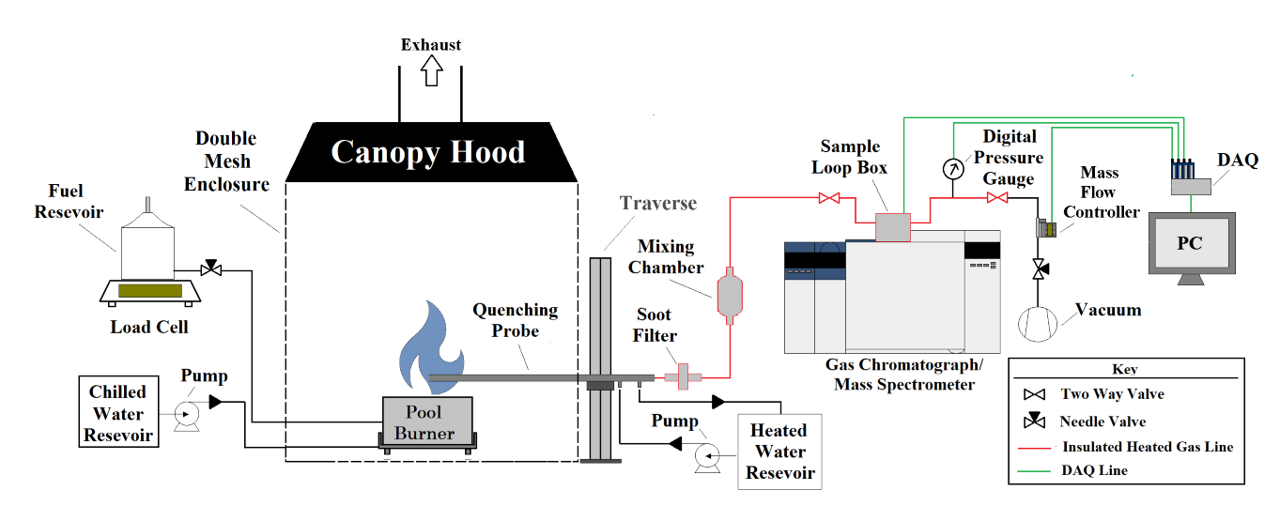
\includegraphics[width=\textwidth,keepaspectratio]{Experimental_Setup.png}
	\caption[A schematic of the gas sampling procedure]{A schematic of the extraction sampling setup used to transport gas samples from the pool fire to the GC/MSD}
	\label{fig:Experimental_Setup}
\end{sidewaysfigure}

Gas sampling was conducted for a minimum of \SI{12.0}{min}, ensuring that the gas sample had completely swept through the GC/MSD sample loop. The gas sampling period varied from \SI{12.0}{min} to \SI{25.0}{min} depending on the sampling location within the fire. The sampling flow was controlled using a mass flow controller (Alicat Scientific MC-Series\footref{fn:product}) located in front of the vacuum pump within the sampling line. During the gas sampling procedure, the volumetric flow was approximately \SI{200.0}{ml/min} and recorded, using a DAQ, at \SI{2.0}{\hertz} for the entire duration of the gas sampling procedure. The mass flow controlled also provided temperature readings of its internal gas flow.

After the gas sampling period, two quarter-turn valves located on opposite ends of the GC/MSD sample loop within the sampling line were closed. Once the sampled gas reached equilibrium, pressure measurements, obtained from a digital pressure gauge (OMEGA DPG409-030DWU\footref{fn:product}), and temperature measurements, acquired by a K-type thermocouple located at the GC/MSD sample loop injection port, were collected at \SI{2.0}{\hertz} for \SI{50.0}{s}. After collecting pressure and temperature measurements, the sampled gas was injected into the GC/MSD.

The volume fraction of a given species, $\bar{X}_{i}$, was calculated from the ratio between the number of moles of a given gas species, $n_{i}$, and the total number of moles identified by the GC/MSD, $n_{tot}$. The total number of moles was determined from the summation of moles for each species identified by either the TCD or MSD.
\begin{equation}\label{eq:volume_fraction}
  	\bar{X}_{i}= \frac{n_{i}}{n_{tot}}
\end{equation}
The mass fraction, $\bar{Y}_{i}$, of a given species $i$ was calculated from the measured volume fraction, $\bar{X}_{i}$, using the following expression:
\begin{equation}\label{eq:mass_fraction}
	\bar{Y}_{i}=\frac{\bar{X}_{i}~{\textrm{MW}_{i}}}{{\textrm{MW}_{tot}}}
\end{equation}
where ${{\textrm{MW}_{i}}}$ is the molecular weight of a given species and ${{MW_{tot}}}$ is the average molecular weight of all detected gas species calculated from Eqn.~\ref{eq:Total_MW}. 
\begin{equation}\label{eq:Total_MW}
	{\textrm{MW}_{tot}}=\sum{\bar{X}_{i}{\textrm{MW}_{i}}}
\end{equation}

All measurements using the GC/MSD were repeated at least twice at each location along the centerline of the pool fire. Gas species concentration measurements made at the same location were averaged. The variance in the gas species volume fraction was a function of position and species. A detailed description of the uncertainty analysis for the gas species measurement and its calibration is discussed in Appendices~\ref{sec:UncertaintyGasSpecies} and \ref{sec:Uncertainty Analysis of Gas Species Calibrations}.

\subsection{Determining Soot Mass Fraction}
\label{ssec:Soot_Setup}

Soot mass fraction, $Y_{s}$, was measured using a well established gravimetric technique~\cite{Choi1995}. Soot was collected simultaneously with gas samples using the sampling procedure described in Section~\ref{ssec:Gas_Species_Setup} and filtered out of the gas stream using a stainless steel particulate filter holder (PALL 2220\footref{fn:product}).  Before a test, a desiccated \SI{47.0}{mm} Polytetrafluoroethylene (PTFE) filter was weighed and subsequently placed into the particulate filter holder. During a test, the filter holder was positioned within the gas sampling line behind the quenching probe and heated to \SI{140.0}{\degree C} using heating tape to prevent condensation of water and liquid fuels on the filter. After testing, the PTFE filter was removed from the filter holder and dried in a dedicator. After dedicating for \SI{48.0}{hrs}, the PTFE filter’s final weight was measured. Approximately \SI{1.0}{mg} of soot was collected during the gas sampling period, which varied from \SI{12.0}{min} to \SI{25.0}{min} depending on the sampling location within the fire.

After some tests, soot deposits were observed on the inner walls of the quenching probe. As shown in Fig.~\ref{fig:Soot_Probe_Setup} dedicated gun cleaning patches were used to clean the inside of the quenching probe. At least two patches were used to collect soot on the inside of the probe. Soot collection on the inside of the probe concluded once an applied patch was observed to have no soot. Patches were weighed immediately before and \SI{48.0}{hrs} after cleaning the inside of the probe. The soot collected from the dry patches was accounted for when calculating the soot mass fraction. The portion of the soot collected on the inner walls of the quenching probe relative to the PTFE filter varied based on the sampling location. The mass of the PTFE filter and cleaning patches were measured three times before and after each test.

\begin{figure}[ht!]
	\centering
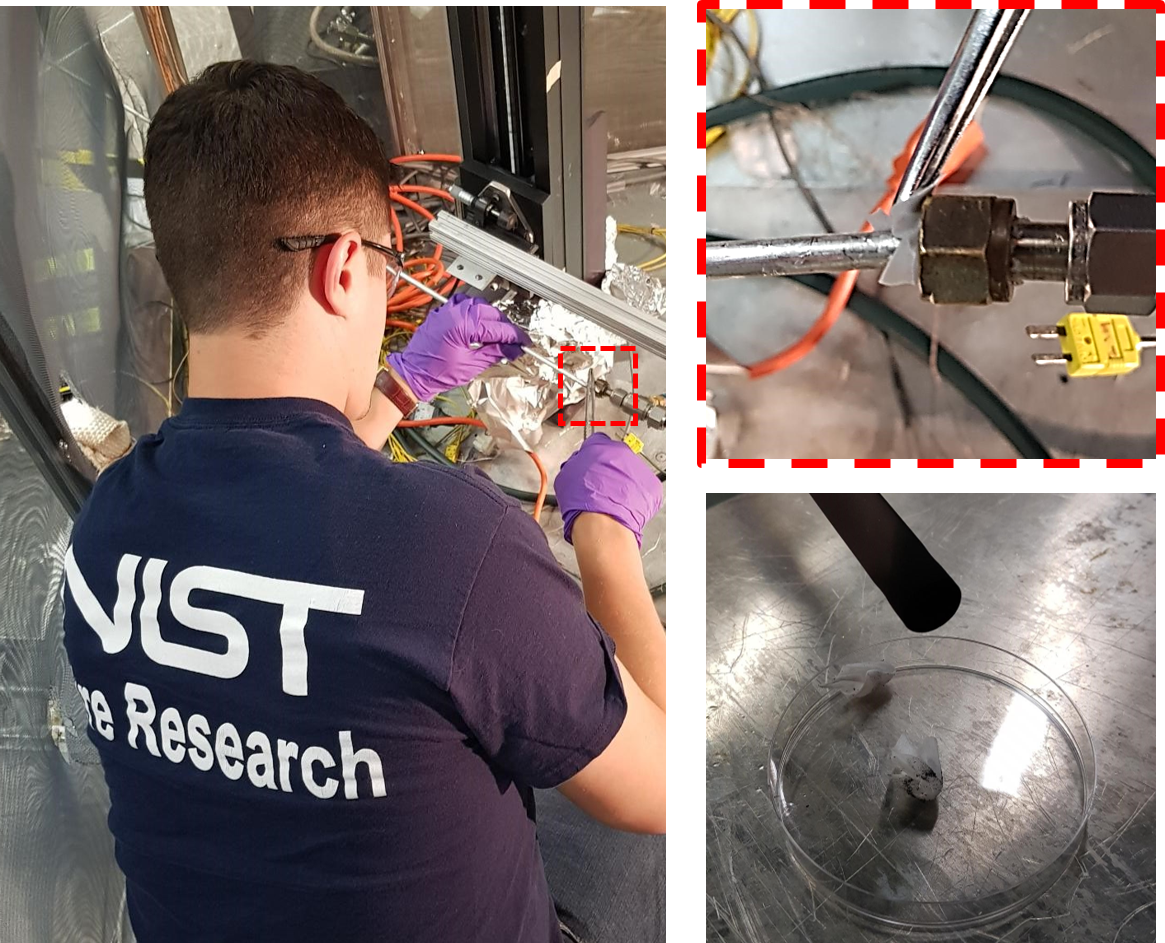
\includegraphics[width=15.0cm,keepaspectratio]{Soot_Probe.png}
	\caption[Process for cleaning soot probe]{Process of collecting soot from the internal walls of the quenching probe using gun cleaning patches}
	\label{fig:Soot_Probe_Setup}
\end{figure}

The soot mass fraction, $m_{s}$, was computed from the mass of the soot collected from the PTFE filter and gun cleaning patches, $m_{s}$, the ratio of the mass flow controller's temperature reading, $T_{\infty}$, to the effective temperature of the gas calculated from Eqn.~\ref{eq:Thermocouple_Bead_Correction}, $T_{g}$, the total mass of gas sampled, $m_{t}$, based on the mass flow controller readings:

\begin{equation}\label{eq:soot_mass_frac}
Y_{s}= \frac{m_{s}}{m_{t}}\frac{T_{\infty}}{T_{g}}
\end{equation}
The total mass of gas sampled was estimated from the product of the average volumetric flow rate measured by the mass flow controller, $\dot{V}$, the density of the sample gas injected into the GC/MSD, $\rho_{g}$, and the gas sampling time, $t$. 
\begin{equation}\label{eq:total_mass}
m_{t}= \dot{V}\cdot \rho_{g}\cdot t
\end{equation} 
In Eqn.~\ref{eq:total_mass}, the density of the sample gas was determined from the total mass detected from the TCD and MSD, $m_{tot}$, for the injected sample volume, $V_{s}$. 
\begin{equation}\label{eq:gas_density}
\rho_{g}= \frac{m_{tot}}{V_{s}}
\end{equation} 
The uncertainty of the soot mass fraction was estimated from a combined uncertainty of the Type A evaluation of standard uncertainty in the variance of temperature and mass measurements and the Type B standard uncertainty in the bias errors of the instrumentation. A detailed description of the soot mass fraction uncertainty is provided in Appendix~\ref{sec:Uncertainty_Soot_Frac}.

\section{Mixture Fraction}
\label{sec:Mixture_Fraction}
The mixture fraction, $Z$, was based on carbon containing species and was defined as follows:
\begin{equation}\label{eq:Mixture_Fraction}
Z=\bar{Y}_{F}+\frac{{\textrm{MW}_{F}}}{x}\sum{\frac{\bar{Y}_{i}}{{\textrm{MW}_{i}}}}
\end{equation} 
where $\bar{Y}_{F}$, ${\textrm{MW}_{F}}$, and $x$ are the mass fraction, molecular weight, and number of carbon molecules of the parent fuel, respectively. The mixture fraction calculation included the mass fraction of soot measured from the technique described in Section~\ref{ssec:Soot_Setup}.
Considering the idealized reaction of a hydrocarbon fuel, the state reactions was derived as:
\begin{align*}
C_{x}H_{y}&O_{z}+\eta(x+\frac{y}{4}-\frac{z}{2})~(O_{2}+3.76~N_{2}+0.0445~Ar)\\
&\rightarrow max(0,1-\eta)~C_{x}H_{y}O_{z}+max(0,1-\eta)~(x+\frac{y}{4}~\frac{z}{2})~O_{2}+ min(1,\eta)~x~CO_{2}\\ 
&~~~~+min(1,\eta)~\frac{y}{2}~H_{2}O+\eta(x+\frac{y}{4}-\frac{z}{2})~(3.76~N_{2}+0.0445~Ar) \numberthis \label{eq:Ideal_rxn}
\end{align*}
where $max(\alpha,\beta)$ and $min(\alpha,\beta)$ are operators that return the larger and smaller value, respectively, of the two parameters $\alpha$ and $\beta$. The parameter $\eta$ represents the portion of air relative to the amount of fuel used as a reactant in Eqn.~\ref{eq:Ideal_rxn}. In other words, $\eta$ can be defined as the reciprocal of the local fuel equivalence ratio, $\phi$,
\begin{equation}\label{eq:Eta}
\phi=\frac{(F/A)}{(F/A)_{st}}=\frac{1}{\eta}
\end{equation} 
where $F/A$ is the fuel-air ratio and the subscript $st$ denotes the stoichiometric condition. The idealized mixture fractions of the products relative to the mixture fraction can then be calculated through a combination of Eqs.~\ref{eq:Mixture_Fraction}, \ref{eq:Ideal_rxn}, and \ref{eq:Eta}. The uncertainty of the mixture fraction was determined from propagating the error in the mass fraction measurements. A detailed description of the mixture fraction uncertainty is provided in Appendix~\ref{sec:Uncertainty_Mix_Frac}. 

\section{Results}
\label{sec:Results}
Brief observations of each pool fire burning different fuels are described in the first portion of this section. The key results of this work are the local gas species and soot measurements made at incremental heights along the centerline of medium-scale pool fires using various fuels such as methanol, ethanol, and acetone. A more in-depth analysis of the relationships between different measured gas is also provided in this section.

\subsection{Flame Observations}
\label{ssec:Flame_Observations}

Figure~\ref{fig:Flame_Structure} displays a series of snapshots depicting the flame pulsation of the methanol, ethanol, and acetone pool fires in the \SI{30}{mm} stainless-steel water-cooled burned. A repeated cycle was observed in each of the pool fires; uniformly curved flame sheets present at the burner rim would roll towards the fire centerline to form a long and narrow plume.
\begin{figure}[!]
	\centering
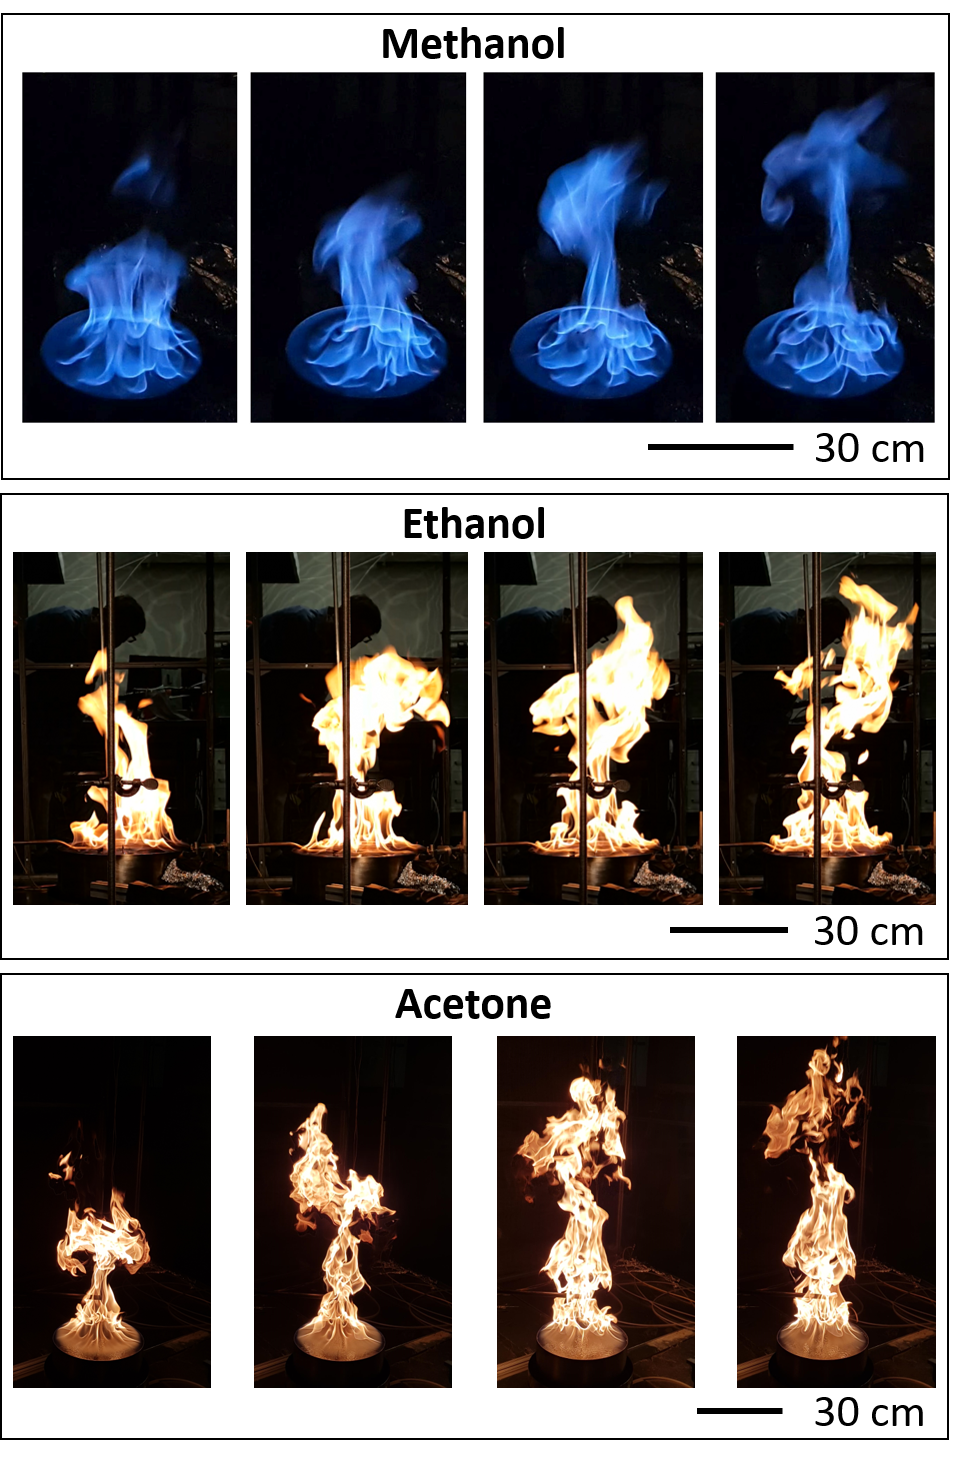
\includegraphics[width=12.0cm,keepaspectratio]{Flame_Structure.png}
	\caption[Pool Fire Structures]{Flame structures of methanol (top), ethanol (middle), and acetone (bottom) pool fires during their pulsing cycles}
	\label{fig:Flame_Structure}
\end{figure}

The shape and visible color of the fires differed between fuel types. The methanol fire appeared to be completely blue, whereas the ethanol, and acetone fires were luminous and yellow. The methanol pool fire was observed to exhibit a quasi laminar flame structure compared to the fully developed fires of the other two fuels. The observed dynamic shapes were consistent with previous experiments~\cite{Hamins2016,Kim2019,Weckman1996,Hamins1994,Hamins1991,Lock2008,Hogben1998}.

The measured time-averaged burning flux and calculated ideal heat release rate are provided in Table~\ref{tab:Pool_Fire_Parameters_Table}. The heat release rate was calculated from Eqn.~\ref{eq:Heat_release_rate}. The time-averaged flame height reported in Table~\ref{tab:Pool_Fire_Parameters_Table}, of the methanol pool fire, was the smallest, followed by the ethanol, and then acetone pool fires. In comparison to the measured mean flame height of each fuel, Heskestad’s theoretical flame height, reported in Ref.~\cite{Heskestad1983}, falls within the experimental uncertainty. The values stated here are in agreement with measurements from~\cite{Kim2019} within the experimental uncertainty.
\begin{table}[!]
\caption{List of measurements and thermochemical properties of fuels burning in a well-ventilated round \SI{30}{mm} diameter pool fire burning in a quiescent environment. The uncertainties of measurements are discussed in detail in Appendix~\ref{sec:Uncertainty_Pool_Fire_Parameters}.}
\label{tab:Pool_Fire_Parameters_Table}
\centering
	\footnotesize
	\begin{tabular}{lccc}
\hline
%\\[0.0005cm]
\textbf{Parameter (units)} &\textbf{Methanol}& \textbf{Ethanol}& \textbf{Acetone}\\
\hline
\\[0.01cm]
Mass Burning Flux~(\si{g/{m^2 s}})		&	12.4~$\pm$~1.1		&	13.9~$\pm$~0.8	&	17.6~$\pm$~2.7\\
\\[0.01cm]
Heat Release Rate~(\si{kW})			&	17.4~$\pm$~1.4		&	26.3~$\pm$~1.5	&	35.5~$\pm$~5.4\\
\\[0.01cm]
Mean Flame Height~(\si{cm})			&	36.4~$\pm$~16.0		&	61.1~$\pm$~28.2	&	91.5~$\pm$~34.6\\
\\[0.01cm]
Heat of Combustion~ (\si{kJ/g})			&	19.9				&	26.8			&	28.6			\\	
\\[0.01cm]
Carbon/Hydrogen 					&	3.0				&	4.0			&	6.0			\\
\hline
\end{tabular}
\end{table}

\subsection{Comparison of Pool Fires from Different Fuels}
\label{ssec:Fuel_comp}
To account for the difference in height between the methanol, ethanol, and acetone pool fires, the mean flame height, $H$, of each fuel was converted to dimensionless distance, $Z^{*}$, that was calculated from Eqn.~\ref{eq:Z_Star}.
\begin{equation}\label{eq:Z_Star}
Z^{*}=H\left(\frac{\dot{Q}}{C_{p}\sqrt{g}\rho_{o}T_{o}}\right)^{\frac{2}{5}}
\end{equation} 
Here $\dot{Q}$ is the heat release rate, $g$ is the gravitational constant, and $C_p$ and $\rho_o$ are the specific heat and the density of air at room temperature, $T_o$. The uncertainty of $Z^{*}$ was calculated from the law of propagation of uncertainty and is detailed in Appendix~\ref{sec:Uncertainty_Z_star}.

Figure~\ref{fig:Temp_Comparison} shows the time-averaged corrected gas temperatures from the centerline of the methanol, ethanol, and acetone pool fires. The maximum mean temperature from each pool fire was found to peak at an approximate $Z^{*}$ of 57. Methanol was determined to have the highest mean temperature of 1316 K with ethanol and acetone exhibiting maximum mean temperatures of 1281 K and 1190 K, respectively. The maximum mean temperature of fuels with higher heat release rates is shown to be lower compared to other fuels. The inverse relationship between heat release rate and maximum mean temperature can be attributed to the radiation loss of the flame to its surroundings. Compared to the raw temperature data, it was discovered that the thermal inertia correction had little influence ($<$ \SI{5}{K}) on the mean temperature but significantly altered the RMS.

\begin{figure}[h!]
	\centering
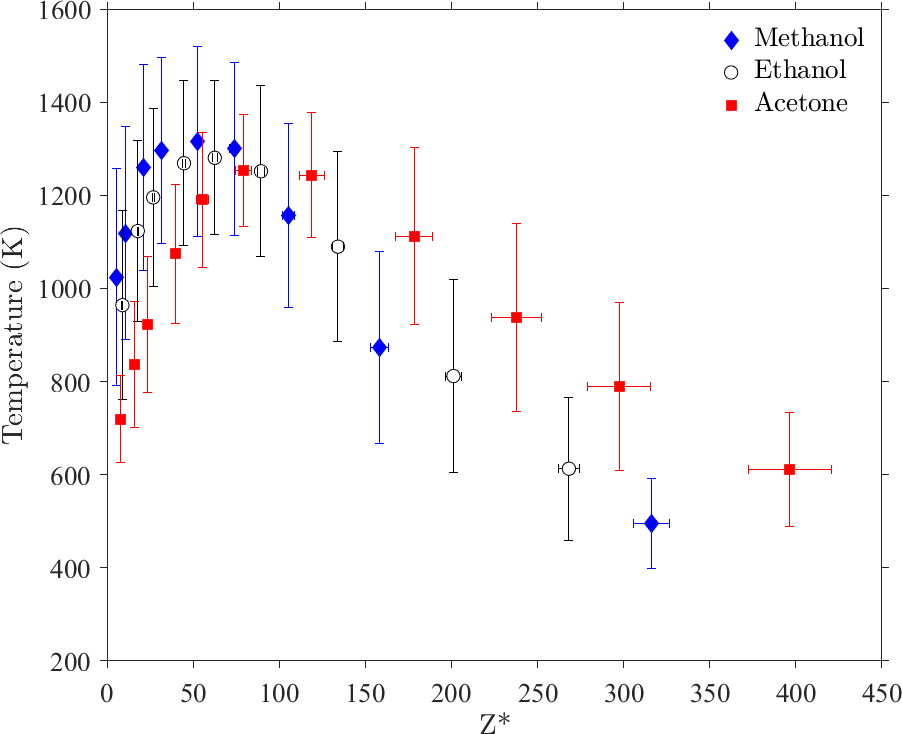
\includegraphics[width=11.0 cm, keepaspectratio]{Temperature_Comparison.png}
	\caption[Major Species Comparison]{Mean and RMS centerline temperature profiles of methanol, ethanol, and acetone pool fires during their pulsing cycles}
	\label{fig:Temp_Comparison}
\end{figure}

Figure~\ref{fig:Fuel_Comparison} displays the volume fraction, $\bar{X}_{i}$, of major species centerline measurements as a function of $Z^{*}$ on the centerline of the methanol, ethanol, and acetone fires. Individual species plots pertaining to each fuel, which shows the major and trace species as a function of $Z^{*}$, are displayed in Appendix~\ref{sec:Vol_Frac_Figs} and include the uncertainty of each measurement. Major species detected in the TCD and MSD include combustion reactants (fuels and oxygen, $\ch{O_2}$), combustion products such as water, $\ch{H_{2}O}$, and carbon dioxide, $\ch{CO_{2}}$, combustion intermediates such as carbon monoxide, $\ch{CO}$, hydrogen, $\ch{H_{2}}$, and inert gases such as Nitrogen, $\ch{N_{2}}$, and Argon, $\ch{Ar}$. Methane was detected and quantified in all fires. In the case of the ethanol and acetone fires, soot, benzene, acetylene, ethylene, and ethane were also detected and quantified. Trace amounts of other species were also detected including propene, acetaldehyde, and ethyl acetate which is consistent with previous literature~\cite{Pichon2009, Gong2015}.

\begin{figure}[!]
	\centering
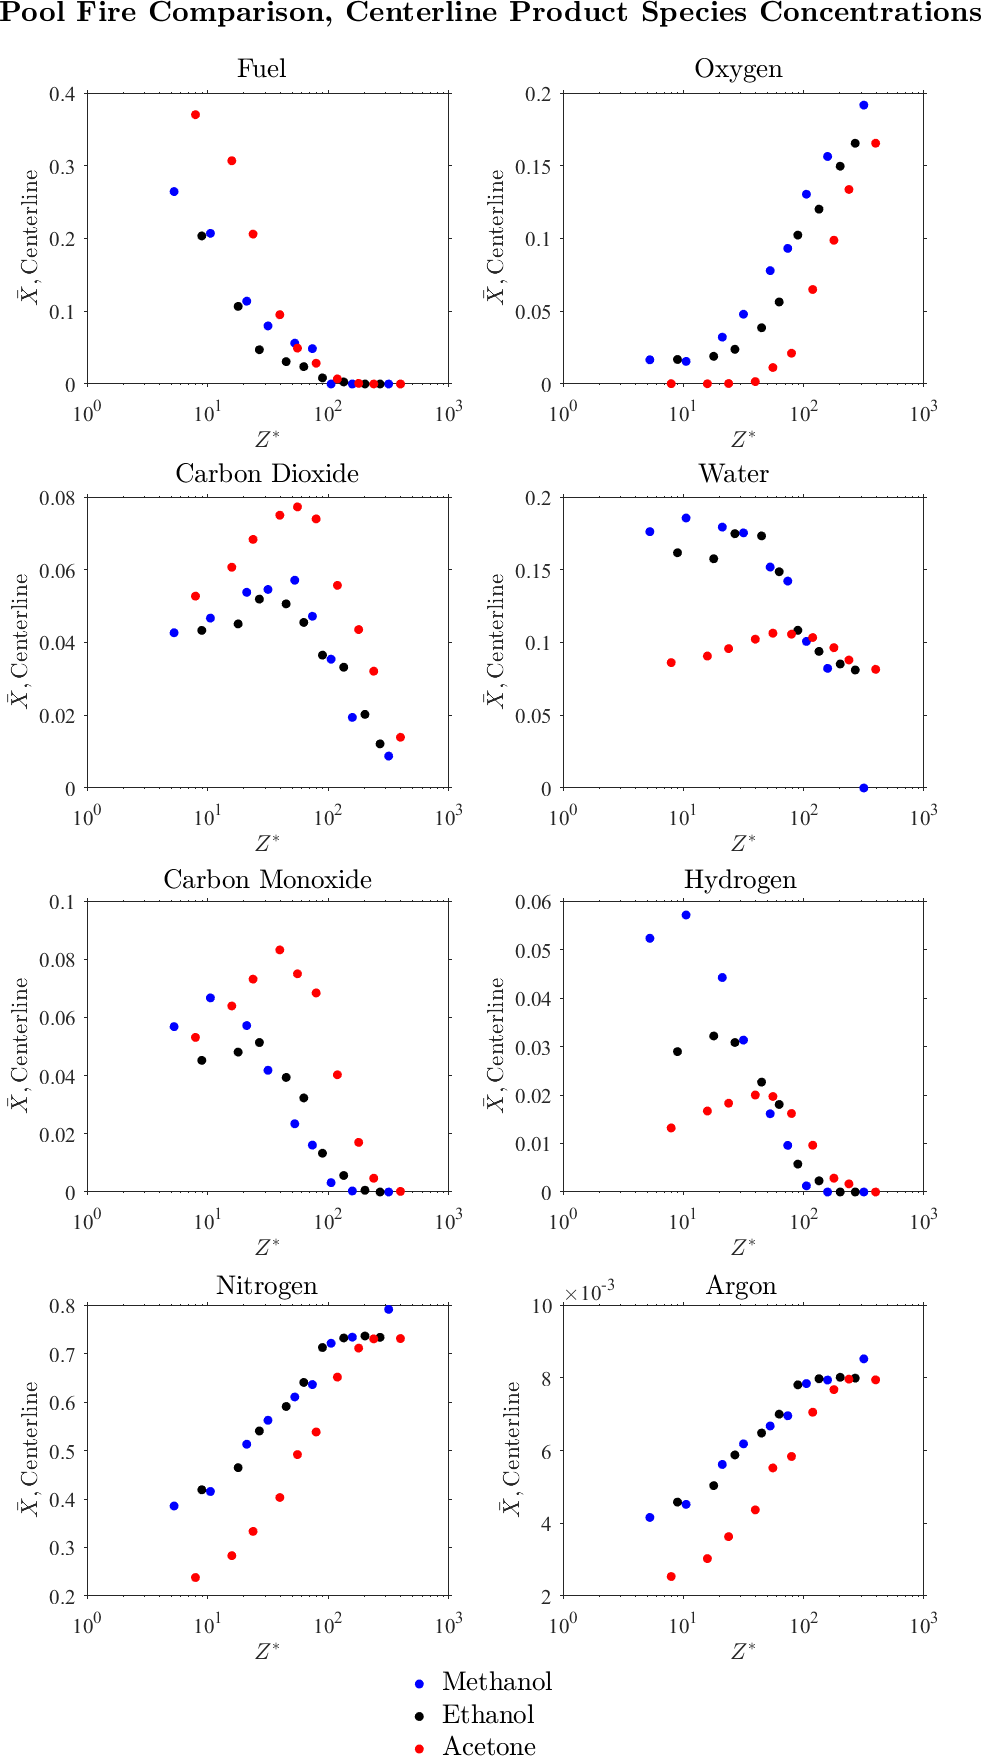
\includegraphics[width=12.5cm,keepaspectratio]{OVERALL_Fuel_Comparison.png}
	\caption[Major Species Comparison]{Centerline volume fraction and soot mass fraction profiles of methanol ($\blacklozenge$), ethanol ($\bigcirc$), and acetone ($\blacksquare$) pool fires.}
	\label{fig:Fuel_Comparison}
\end{figure}

For all fuels, the fuel and oxygen volume fractions were highest and lowest, respectively, close to the fuel surface. Furthermore, the volume fractions of inert gases were found to have increased relative to the distance from the fuel surface. Methanol and ethanol volume fractions profiles of $\ch{H_{2}O}$, $\ch{CO_{2}}$, and $\ch{CO}$, with respect to $Z^{*}$ were reasonably similar. The largest volume fractions of all product species, such as $\ch{CO_2}$, $\ch{CO}$, and $\ch{H_2O}$ was achieved when burning acetone, except for $\ch{H_{2}}$ in which its peak was determined to be the lowest compared to the other fuels. Acetone was also found to produce a greater mass fraction of soot at every location of the centerline profile compared to the ethanol fire.

\subsection{Mixture Fraction Results}
\label{ssec:Mixture_Fraction_Results}
In this section, the results of the fuels are presented corresponding to fuel type, since fuel type established the relationship between mass and mixture fraction as defined in Eqn.~\ref{eq:Mixture_Fraction}. Figures~\ref{fig:Methanol_Mix_Frac}, \ref{fig:Ethanol_Mix_Frac}, and \ref{fig:Acetone_Mix_Frac} show the averaged quasi-steady mass fractions measurements as a function of the mixture fraction for the methanol, ethanol, and acetone fires, respectively. The dotted lines in each of the figures represent idealized combustion calculated from Eqs.~\ref{eq:Mixture_Fraction}, \ref{eq:Ideal_rxn}, and \ref{eq:Eta}, in that it is assumed that no intermediate species (i.e., $\ch{CO}$, $\ch{H_{2}}$, or soot) are produced. The vertical dotted line defines the stoichiometric combustion condition of which to its left and right represents the fuel-lean ($Z<Z_{st}$) and fuel-rich ($Z>Z_{st}$) regions, respectively. In all figures, the vertical error bars represent the propagated uncertainty of the averaged mass fractions. Additional plots that detail the averaged mass fractions of all detected species as a function of mixture fraction, with their expanded uncertainties, are provided in Appendix~\ref{sec:Mix_Frac_Figs}. 

\begin{figure}[!]
	\centering
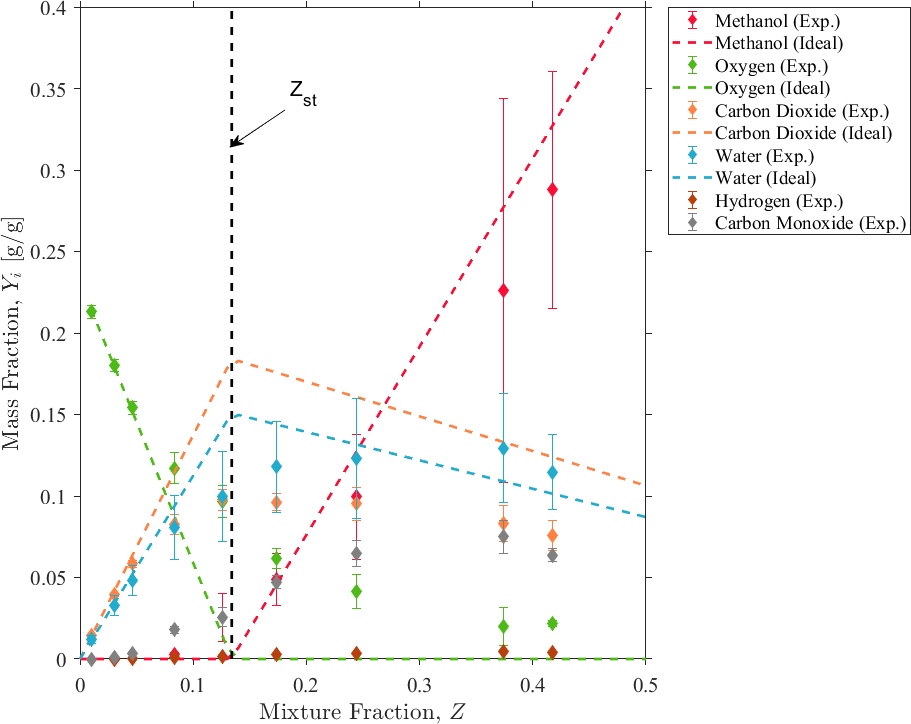
\includegraphics[width=11.0cm,keepaspectratio]{Methanol_OVERALL_Mass_Frac_Mix_Frac.png}
	\caption[Averaged quasi-steady mass fraction of major species as a function of mixture fraction for a \SI{30}{cm} methanol pool fire]{Averaged quasi-steady mass fraction of major species as a function of mixture fraction for a \SI{30}{cm} methanol pool fire}
	\label{fig:Methanol_Mix_Frac}
\end{figure}

\begin{figure}[!]
	\centering
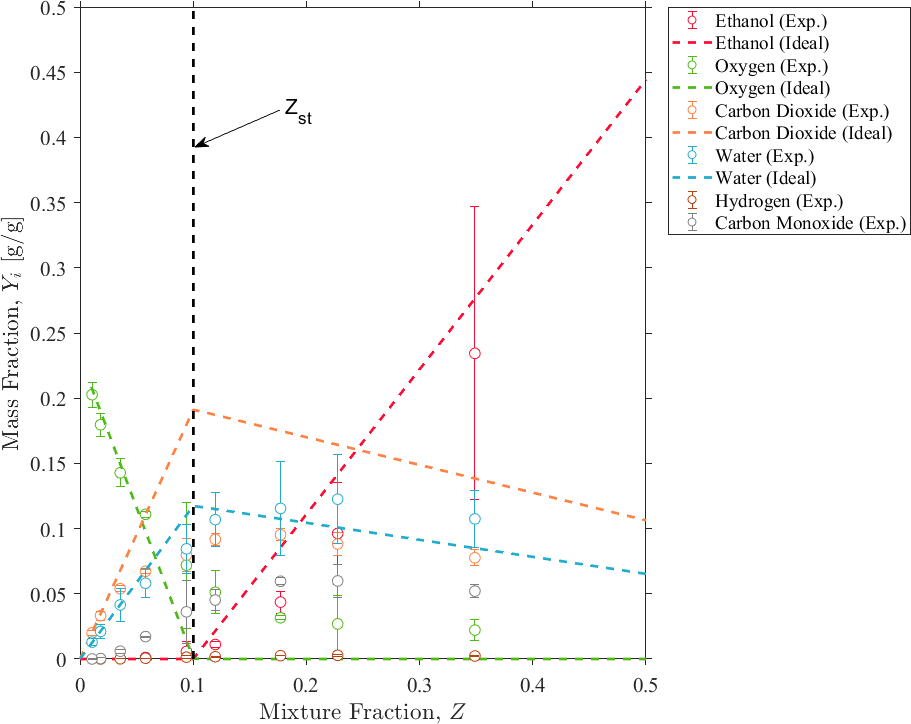
\includegraphics[width=11.0cm,keepaspectratio]{Ethanol_OVERALL_Mass_Frac_Mix_Frac.png}
	\caption[Averaged quasi-steady mass fraction of major species as a function of mixture fraction for a \SI{30}{cm} ethanol pool fire]{Averaged quasi-steady mass fraction of major species as a function of mixture fraction for a \SI{30}{cm} ethanol pool fire}
	\label{fig:Ethanol_Mix_Frac}
\end{figure}

\begin{figure}[!]
	\centering
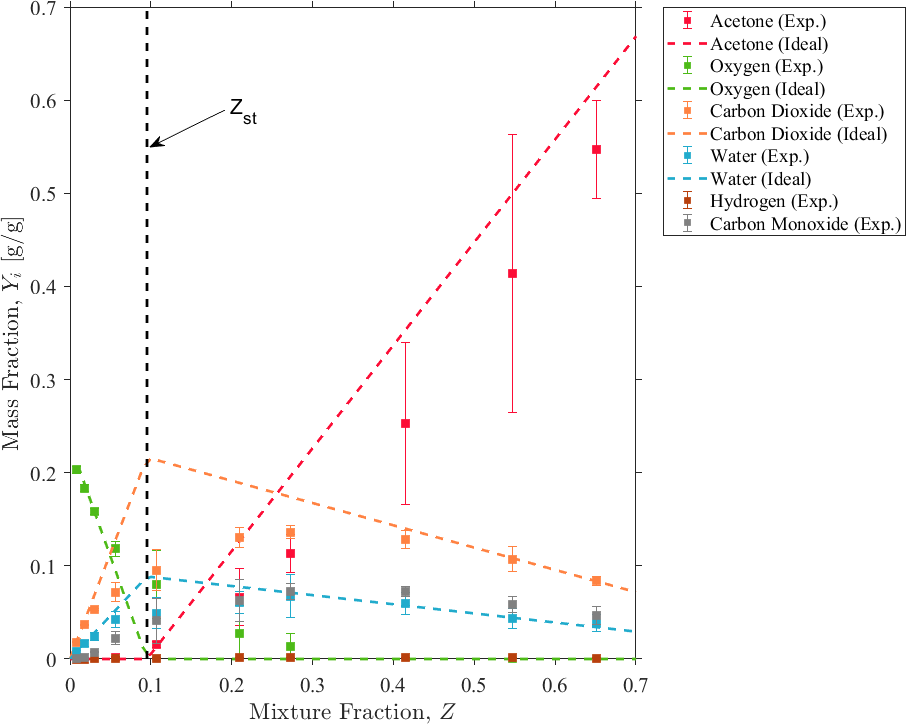
\includegraphics[width=11.0cm,keepaspectratio]{Acetone_OVERALL_Mass_Frac_Mix_Frac.png}
	\caption[Averaged quasi-steady mass fraction of major species as a function of mixture fraction for a \SI{30}{cm} acetone pool fire]{Averaged quasi-steady mass fraction of major species as a function of mixture fraction for a \SI{30}{cm} acetone pool fire}
	\label{fig:Acetone_Mix_Frac}
\end{figure}

In the instances where the mixture fraction is small ($Z<<Z_{st}$), all major gas species are in fair agreement with the theoretical lines; the measured mass fractions of unburned fuel and $\ch{CO}$ are nearly zero, and the $\ch{O_2}$ is close to its respective theoretical value. As the mixture fraction approaches stoichiometric conditions, the measured mass fraction of $\ch{O_{2}}$ decreases while $\ch{CO_{2}}$ and $\ch{H_{2}O}$ increases. The measured mass fraction of $\ch{CO_{2}}$ and $\ch{H_{2}O}$ are found to peak close to the stoichiometric mixture fraction. As the mixture fraction increases past the stoichiometric condition, the measured mass fraction of the unburned fuel is shown to increase, following the same trend as the idealized case. In the fuel-rich regions, the measured mass fraction of $\ch{CO_{2}}$ differs considerably from the theoretical case. The difference between the measured $\ch{CO_{2}}$ concentration and the theoretical value is attributed to the substantial portion of $\ch{CO}$, which exhibits a comparable trend to $\ch{CO_{2}}$ with respect to the mixture fraction. The presence of soot and other carbon containing species also attributes to the under-predicted concentration of $\ch{CO_{2}}$ relative to the theoretical case. 

\subsection{Verifying Gas Species Measurements}
\label{ssec:Verifying_Vol_Frac_Measurements}
As a way to verify the accuracy of the experimental method, specifically the calibration procedure and curve fit, the total moles identified, $n_{tot}$, by the TCD and MSD was compared to the total moles injected into the GC/MSD system. The total moles injected, $n_{inj}$, into the GC/MSD was calculated from the ideal gas equation, Eqn.~\ref{eq:moles_inj}.
\begin{equation}\label{eq:moles_inj}
n_{inj}=\frac{PV_{sl}}{RT}
\end{equation} 
Here, $R$ is the universal gas constant (287~J/(mol $\cdot$K), $V_{sl}$ is the volume of the GC/MSD sample loop (\SI{2.0}{ml}), and $P$ and $T$ are the averaged pressure and temperature measurements, respectively, collected before injecting the gas sample into the GC/MSD as described in Section~\ref{ssec:Gas_Species_Setup}. The combined uncertainty of the total moles injected is detailed in Section~\ref{ssec:Total Moles Injected into the GC/MSD for Calibation}.

\begin{figure}[h!]
	\centering
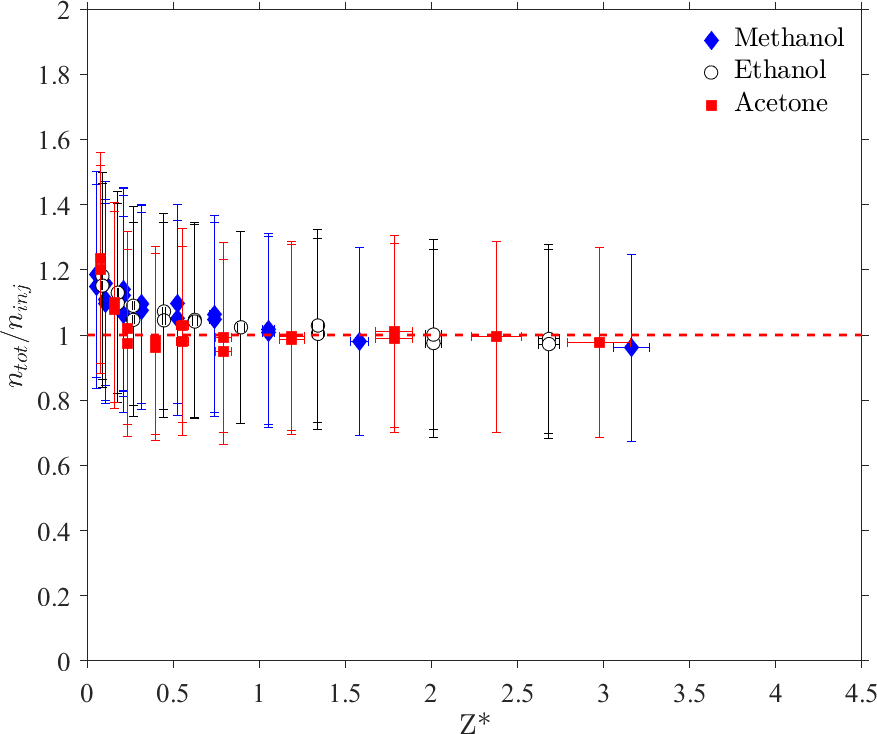
\includegraphics[width=10.5cm,keepaspectratio]{mole_ratio_Comparison.png}
	\caption[Ratio of moles identified to moles injected, with error, as a function of $Z^{*}$]{Ratio of moles identified to moles injected, with error, as a function of $Z^{*}$ compared to the theoretical value}
	\label{fig:Mole_Comp}
\end{figure}

Figure~\ref{fig:Mole_Comp} shows the ratio of the moles identified by the TCD and MSD to the mole injected into the GC/MSD as a function of $Z^{*}$. The horizontal dotted line represents the theoretical instance when the moles identified is equal to the moles injected. In most cases, the ratio is close to unity, indicating that the total moles injected into the GC/MS are all accounted for in the calculation. In some instances, where $Z^{*}$ is small ($<35$), the ratio is higher than the theoretical value. This difference indicates an error in the calibration, which is over predicting certain gas species; most likely fuel species since there are high concentrations of fuel close to the fuel surface. The discrepancy between the measured and theoretical values is accounted for in the uncertainty as shown in the error bars which extend beyond the unity line. 

Another way to verify the accuracy of the gas species measurements was to calculate the carbon to hydrogen, product species, and inert species ratios from the methanol, ethanol, and acetone pool fires. Each calculation only incorporates quantified species and assumes other identified species are trace amounts. The expanded uncertainty of the carbon to hydrogen, product, and inert ratios was determined using the law of propagation of uncertainty that accounted for the error of each species' volume fraction measurement and discussed in Appendix~\ref{sec:Uncertainty_Ver_Scheme}. 

The theoretical value of the carbon to hydrogen ratio was determined from the mass fraction of carbon and hydrogen residing within the parent fuel and are reported in Table~\ref{tab:Pool_Fire_Parameters_Table}. As shown in Eqn.~\ref{eq:c2h_ratio} the carbon to hydrogen ratio was calculated from the mass fraction of any quantified gas species that contained either carbon, $\bar{Y}_{i,C}$, or hydrogen, $\bar{Y}_{i,H}$. Here $\textrm{MW}_{C}$ and $\textrm{MW}_{H}$ are the molecular weights of carbon and hydrogen.

\begin{equation}\label{eq:c2h_ratio}
 \frac{C}{H}=\frac{\sum{\bar{Y}_{i,C}~{\frac{\textrm{MW}_{C}}{\textrm{MW}_{i,C}}}}}{\sum{\bar{Y}_{i,H}~{\frac{\textrm{MW}_{H}}{\textrm{MW}_{i,H}}}}}
\end{equation}

The carbon to hydrogen ratio for each experiment is shown in Fig.~\ref{fig:C2H}. The dotted line represents the theoretical value stated in Table~\ref{tab:Pool_Fire_Parameters_Table}. For each fuel, the data is shown to be in agreement with the theoretical value indicating that the analysis is successful in quantifying most of the carbon and hydrogen containing species.   

\begin{figure}[h!]
	\centering
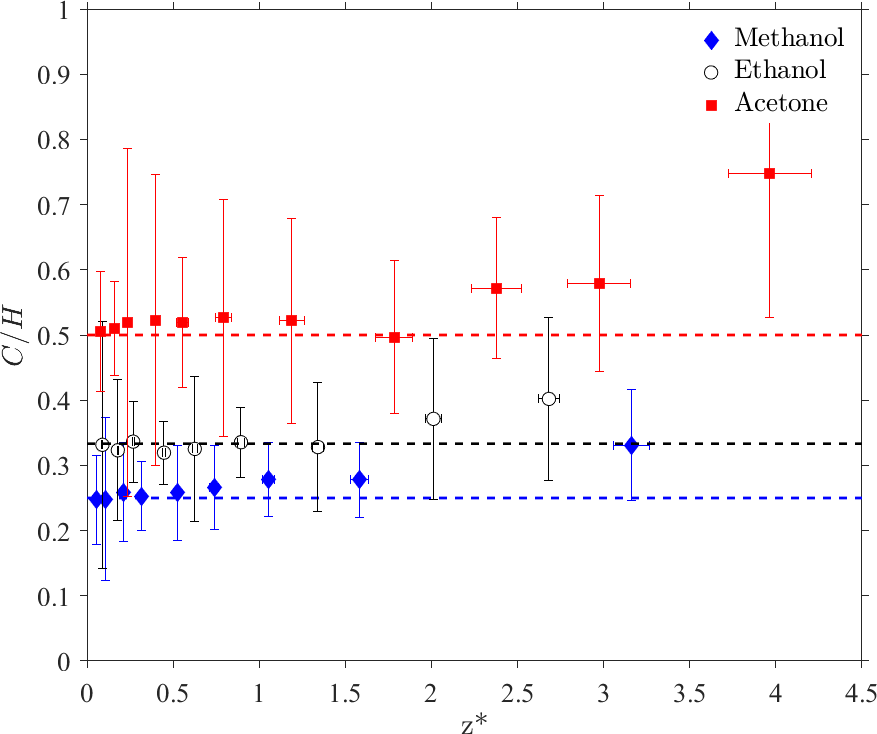
\includegraphics[width=10.5cm, keepaspectratio]{C2H_ratio_Comparison.png}
	\caption[Carbon to hydrogen ratio calculated from experimental values compared to theoretical values]{Carbon to hydrogen ratio calculated from experimental values with error compared to theoretical values. Dotted lines represent the theoretical carbon to hydrogen ratio calculated from the mass fraction of carbon and hydrogen residing within the parent fuel}
	\label{fig:C2H}
\end{figure}

Another verification test was comparing volume fraction measurements to stoichiometric combustion ratios, $\text{SCR}$, determined from the reaction below.
\begin{align*}
C_{x}H_{y}&O_{z}+a~(O_{2}+3.76~N_{2}+0.0445~Ar)\\
&\rightarrow b~C_{x}H_{y}O_{z}+c~O_{2}+ d~CO_{2}+e~H_{2}O+f~H_{2}+ g~CO\\
&~~~~+h~CH_{4}+ i~C_{2}H_{2}+j~C_{2}H_{4}+k~C_{2}H_{6}+l~C_{6}H_{6}\\
&~~~~+f~(3.76~N_{2}+0.0445~Ar) \numberthis \label{eq:Ideal_rxn}
\end{align*}
When simplified, the $\text{SCR}$ of each fuel was calculated as:
\begin{equation}\label{eq:prod_ratio_methanol}
 \text{SCR}_{methanol}=\frac{\bar{X}_{H_2O}+\bar{X}_{H_2}}{\bar{X}_{CO_2}+\bar{X}_{CO}}=2
\end{equation}
\begin{equation}\label{eq:prod_ratio_ethanol}
\text{SCR}_{ethanol}=\frac{\bar{X}_{H_2O}+\bar{X}_{H_2}+\frac{1}{2}\bar{X}_{CH_4}}{\bar{X}_{CO_2}+\bar{X}_{CO}+\frac{2}{3}(\bar{X}_{C_2H_4}+2\bar{X}_{C_2H_2})+4\bar{X}_{C_6H_6}}=\frac{3}{2}
\end{equation}
\begin{equation}\label{eq:prod_ratio_acetone}
\text{SCR}_{acetone}=\frac{\bar{X}_{H_2O}+\bar{X}_{H_2}+\bar{X}_{CH_4}+\bar{X}_{C_2H_6}}{\bar{X}_{CO_2}+\bar{X}_{CO}+\bar{X}_{C_2H_2}+3\bar{X}_{C_6H_6}}=1
\end{equation}
The derivation for methanol, ethanol, and acetone's SCRs is provided in Appendix~\ref{sec:SCR_Derv}.

Figure~\ref{fig:SCR} shows the difference between the $\text{SCR}$ and experimental data. The dotted lines represents the $\text{SCR}$ values calculated from Eqns.~\ref{eq:prod_ratio_methanol}, \ref{eq:prod_ratio_ethanol}, and \ref{eq:prod_ratio_acetone}. Direct comparison of the measured values to the idealized values shows that there is general agreement and that the volume fraction measurements are not unreasonable. An exact match is not expected since the idealized values do not take into account molecular diffusion, nor the mass of soot. 
\begin{figure}[h!]
	\centering
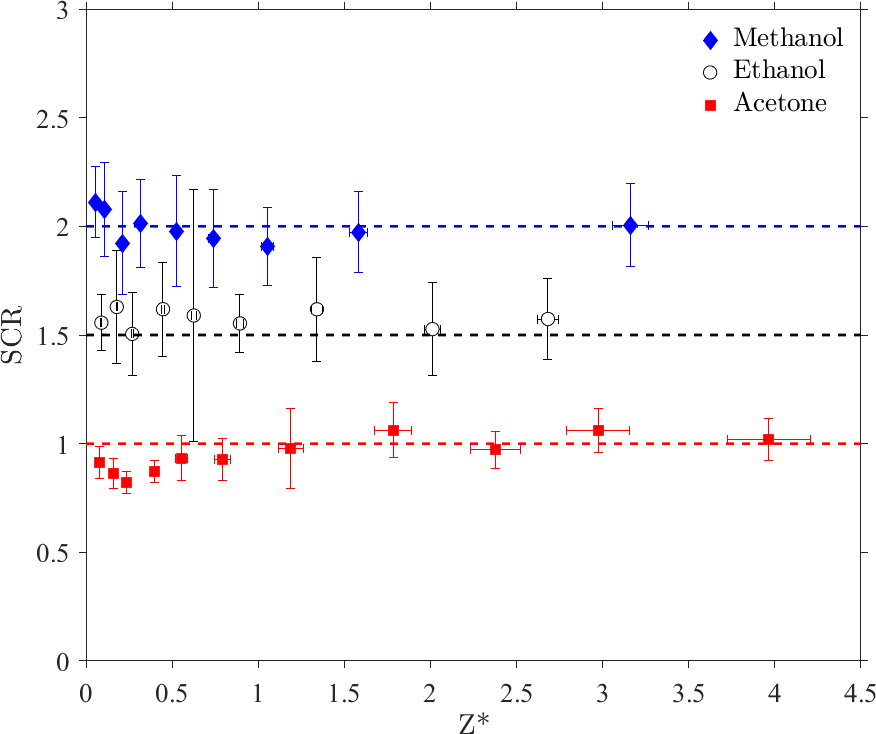
\includegraphics[width=10.5cm, keepaspectratio]{Prod_ratio_Comparison.png}
	\caption[Stoichiometric Combustion Ratio calculated from experimental values compared to theoretical values]{Comparison of Stoichiometric Combustion Ratio, $\text{SCR}$, calculated from experimental and theoretical values compared to theoretical values. Dotted lines represent the theoretical $\text{SCR}$ calculated using Eqns.~\ref{eq:prod_ratio_ethanol}, \ref{eq:prod_ratio_methanol}, \ref{eq:prod_ratio_acetone}.}
	\label{fig:SCR}
\end{figure}

An inert ratio was also calculated from the volume fraction measurements of argon to nitrogen. Since both argon and nitrogen are inert, the ratio between them should be reasonably consistent across all fuels. The inert ratio was measured from ambient air samples using the setup described in Sec.~\ref{ssec:Gas_Species_Setup}. The inert ratio of ambient air was determined to be $0.012~\pm~4~\%$. The range of the inert ratios calculated from the ambient air sample is depicted in Fig.~\ref{fig:IR} as the error band. The error band is shown to extend beyond all calculated inert ratios, which further supports the validity of the measurements. 
\begin{figure}[h!]
	\centering
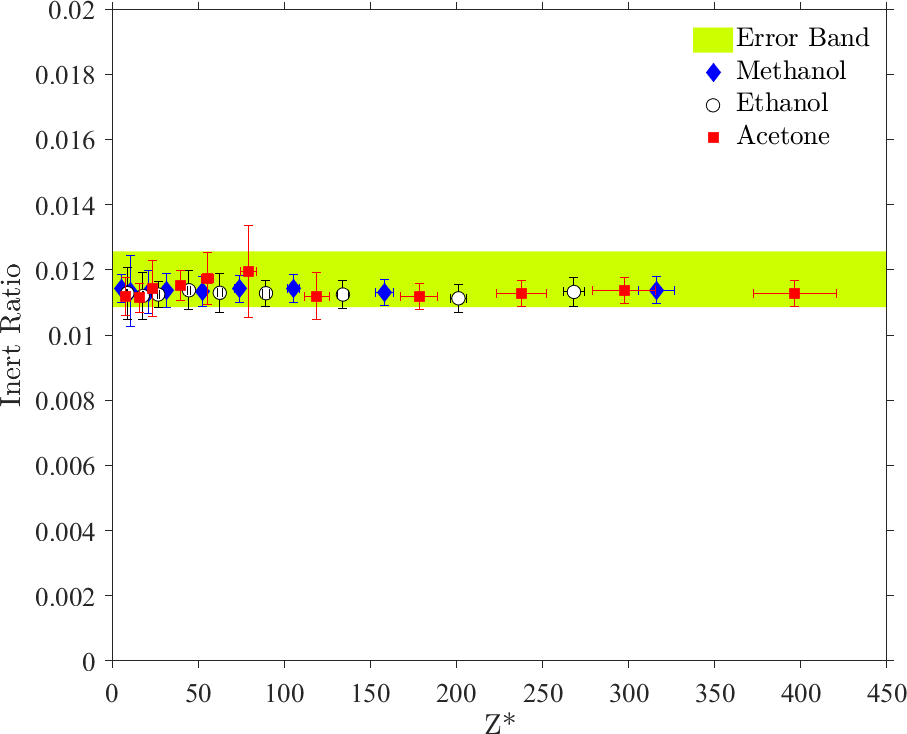
\includegraphics[width=10.5cm, keepaspectratio]{Inert_ratio_Comparison.png}
	\caption[Stoichiometric Combustion Ratio calculated from experimental values compared to theoretical values]{Inert ratios calculated from the volume fractions of argon and nitrogen compared to inert ratios determined from ambient air and represented as error band.}
	\label{fig:IR}
\end{figure}


\section{Conclusion}
\label{sec:Conclusion}
In summary, time-averaged local measurements of temperature and gas species concentrations were made to characterize the structure of methanol, ethanol, and acetone \SI{30}{cm} diameter pool fire steadily burning in a quiescent environment. A verification scheme was developed to verify the gas species measurements that considered  the accuracy of the calibration and the overall stoichiometry of combustion for each fuel (see Eqn.~\ref{eq:prod_ratio_ethanol}, \ref{eq:prod_ratio_methanol}, and \ref{eq:prod_ratio_acetone}). The gas species measurements were favorably compared to the idealized SCR values, which lends confidence to the veracity of the measurements. These local measurements complement previous measurements and provide insight into the complex chemical structure of medium-scale pool fires.

\section*{Acknowledgments}
\noindent The authors would like to acknowledge Kimberly Harris of the Gas Sensing Metrology Group at NIST, who assisted in the developing the species calibration method used in the study.
\pagebreak

\section*{References}
\addcontentsline{toc}{section}{References}
\bibliographystyle{techpubs}
\bibliography{References}
\pagebreak


\appendix
\numberwithin{equation}{section}
\makeatletter
% "activate" the preparatory code, but for section-level headers only
\newcommand{\section@cntformat}{Appendix:\ }
\makeatother

\section{Uncertainty Analysis of Pool Fire Parameters}\label{sec:Uncertainty_Pool_Fire_Parameters}
\addcontentsline{toc}{section}{Appendix A: Uncertainty of Pool Fire Parameters}

\subsection{Mass Burning Rate}
\label{ssec:Mass_Burning_Flux}
The mass burning rate, $\dot{m}$, was measured from the mass loss in the fuel reservoir, feeding to the pool burner via gravity, during the burning period per area of the pool burner. Mass measurements were made using a Precisa XB-6200C Precision XB Laboratory Prime Balance sampling at \SI{1.0}{\hertz} for the entire duration of the burning period. The balance was calibrated from a collection standard weights. The expanded uncertainty was estimated via quadrature from a combination of the Type A and Type B evaluation of standard uncertainty. The Type A evaluation of standard uncertainty was calculated from the standard error, $s_{\scriptscriptstyle \dot{m}}$, of the time-averaged mass loss measured during the burning period. The Type B evaluation of standard uncertainty was determined from the bias error of the balance, $u_{\rm \scriptscriptstyle inst}$ (\SI{0.01}{g}), and the calibration error, $u_{\rm \scriptscriptstyle cal}$ (1~\% of the reading).

\begin{equation}
\label{eq:mass_rate_uncertainty}
u_{\scriptscriptstyle \dot{m}} = \sqrt{s_{\scriptscriptstyle \dot{m}}^2+u_{\rm \scriptscriptstyle inst}^2+u_{\rm \scriptscriptstyle cal}^2}
\end{equation}
 
\subsection{Heat Release Rate}
\label{ssec:Heat_Release_Rate}
The heat release rate was determined from Eqn.~\ref{eq:Heat_release_rate} using the heat of combustion property of the respective fuel, provided by DIPPR\textsuperscript{\textregistered}, and time-averaged mass burning rate values listed in Table~\ref{tab:Pool_Fire_Parameters_Table}. The uncertainty of the heat release rate was calculated via the law of propagation of uncertainty:

\begin{equation}
\label{eq:heat_release_rate_uncertainty}
u_{\scriptscriptstyle \dot{Q}} = \sqrt{{\left(\frac{\partial \dot{Q}}{\partial \dot{m}}\,u_{\scriptscriptstyle \dot{m}} \right)}^2}
\end{equation}
The description of the mass burning rate uncertainty is provided in Appendix~\ref{ssec:Heat_Release_Rate}.

\subsection{Mean Flame Height}
\label{ssec:Mean_Flame_Height}
The mean flame height, $u_{h_{f}}$, was determined by measuring the distance between the pool surface and flame tip using the photographic analysis method described in Section~\ref{ssec:Pool_Burner_Setup}. The uncertainty of the mean flame height, $u_{\scriptscriptstyle h_{fl}}$, was calculated from a combined uncertainty of the Type A and B evaluation of standard uncertainty. The Type A evaluation of standard uncertainty was estimated from the standard deviation of the height measurements, $s_{\scriptscriptstyle h_{fl}}$, made with each frame. The error of the measured distance using the photographic analysis method compared to the true distance, $u_{\scriptscriptstyle meth}$,  was found to be 0.1\% and was treated as the Type B evaluation of standard uncertainty. The combined uncertainty calculation of the mean flame height is shown below:

\begin{equation}
\label{eq:mean_flame_height}
u_{\scriptscriptstyle h_{f}} = \sqrt{s_{\scriptscriptstyle{h_{f}}}^2+u_{\rm \scriptscriptstyle meth}^2}
\end{equation}

\pagebreak

\section{Uncertainty Analysis of Temperature Measurements}\label{sec:Uncertainty_Temperature_Measurements}
\addcontentsline{toc}{section}{Appendix B: Uncertainty of Temperature Measurements}

Temperature measurements were sampled at \SI{250.0}{Hz} for \SI{2.0}{min} using a S-type (Pt 10\% Rh/Pt), bare-wire, fine diameter thermocouple with a diameter of \SI{50.0}{\micro\metre} (OMEGA P10R-001\footref{fn:product}). Temperature measurements were corrected for following Shassix's method~\cite{Shaddix1999} and using Eqn.~\ref{eq:Thermocouple_Bead_Correction}:
\begin{equation}\label{eq:Thermocouple_Bead_Correction_full}
{T_{g}(t)}= T_{b}(t)+{\frac{\rho_{b}c_{p,b}{d_{b}}^2}{6Nu\lambda_{g}}}\frac{dT_{b}}{dt}+\frac{\epsilon\sigma d_{b}}{Nu \lambda_{g}}\left({T_{b}(t)}^4-{T_{surr}(t)}^4\right)
\end{equation}
where $T_{g}$ is the effective temperature of the gas, $T_{surr}$ is the effective temperature of the surroundings, $\lambda_{g}$ is the thermal conductivity of the gas, $Nu$ is the Nusselt number calculated from Eqn.~\ref{eq:Nu_number}, $\sigma$ is the Stefan-Boltzmann constant (\SI{5.6696E-8}{W/(m^2~K^4}), $\epsilon$ is the thermocouple emmisivity, and $T_{b}$, $\rho_{b}$, $c_{p,b}$, $d_{b}$ are the raw temperature measurements, density, specific heat, and diameter of the bead, respectively. The uncertainty of the effective temperature of the gas was calculated from the uncertainty of all temperature dependent parameters included in Eqn.~\ref{eq:Thermocouple_Bead_Correction_full}. The temperature dependent variables included in Eqn.~\ref{eq:Thermocouple_Bead_Correction_full} are $\lambda_{g}$, $Nu$, $\epsilon$, $T_{b}$, $\rho_{b}$, $c_{p,b}$ whereas all other parameters are considered as constant. The uncertainty of the corrected temperature measurements were estimated using a propagation of uncertainty:
 \begin{equation}
\label{eq:temperature_corr_uncer}
u_{\scriptscriptstyle T_{g}} = \sqrt{{\left(\frac{\partial T_{g}}{\partial T_{b}}\,u_{\scriptscriptstyle T_{b}} \right)}^2}
\end{equation}

\subsection{Uncertainty of Bead Temperature Measurements}
\label{ssec:Uncertain_Bead_Temp_Measurements}
The uncertainty of the raw bead temperature measurements was calculated from a combined Type A and B evaluation of uncertainty. The Type A evaluation of raw bead temperature measurements was determined from the standard error of temperature, $s_{T}$ readings from the sampling period. The Type B evaluation of uncertainty for the raw bead temperature measurements was determined from the bias error sources in the instrumentation, $u_{inst}$, used to measure temperature (\SI{1.5}{\degree C}) of gas sample injected. The combined uncertainty temperature was found via quadrature:

\begin{equation}
\label{eq:temp_uncertainty}
u_{\scriptscriptstyle T_{b}} = \sqrt{ u_{\rm \scriptscriptstyle inst}^2 + s_{\scriptscriptstyle T_{b}}^2}
\end{equation}
\pagebreak

\section{Uncertainty Analysis of Gas Species Concentrations} \label{sec:UncertaintyGasSpecies}
\addcontentsline{toc}{section}{Appendix C: Uncertainty Analysis of Gas Species Concentrations}

\subsection{Uncertainty of Volume Fractions} \label{sec:UncertaintyMoleFrac}
As shown in Eqn.~\ref{eq:volume_fraction}, volume fraction, $\bar{X}_{i}$, was calculated from the ratio between the number of moles of a given species, $n_{i}$, and the total number of moles identified, $n_{tot}$. The uncertainty of the measured volume fraction was estimated using the law of propagation of uncertainty after determining the volume fraction of each species:

\begin{equation}
\label{eq:Volume_Frac_Uncertainty}
u_\mathrm{\bar{X}_{i}} = \sqrt{{\left( \frac{\partial \bar{X}_{i}}{\partial n_{i}}\,u_{\scriptscriptstyle n_{i}} \right)}^2+{\left(\frac{\partial \bar{X}_{i}}{\partial n_{tot}}\,u_{\scriptscriptstyle n_{tot}}\right)}^2}
\end{equation}
A coverage factor of 2 was applied to the combined uncertainty to produce a 95~\% confidence interval.

\subsubsection{Number of Moles of a Given Species}
\label{ssec:Number_of_Moles_of_a_Given_Species}

The number of moles of a given species was determined from a calibration function of the integrated peak area of the respective species obtained from the TCD's and the MSD's Total Ion Current (TIC) chromatograms. The Type A evaluation of standard uncertainty of the number of moles of a given species was taken as the standard deviation of the measurements obtained from the repeated tests. The Type B evaluation of standard uncertainty was determined from the error in the calibration functions for each species measured by the TCD and MSD is further detailed in Appendix~\ref{sec:Uncertainty Analysis of Gas Species Calibrations}. The combined uncertainty was found via quadrature:

\begin{equation}
\label{eq:gasspeciesuncertaintycertainty}
u_{\scriptscriptstyle n_{i}} = \sqrt{ u_{\rm \scriptscriptstyle n_{i,cal}}^2 + s_{\scriptscriptstyle n_{i}}^2}
\end{equation}

\subsubsection{Total Number of Moles Identified}
\label{ssec:Total Number of Moles Identified}
The total number of moles detected was determined from the summation of the number of moles for each species identified by the TCD and TIC chromatograms. Therefore, the uncertainty in the total number of moles identified was the combined uncertainty of all the identified species via quadrature:

\begin{equation}
\label{eq:totalnumberofmolesdetected}
u_{\scriptscriptstyle n_{tot}}=\sqrt{{\sum_{n=1}^{N} s_{\scriptscriptstyle n_{i}}^2}}
\end{equation}
where $N$ is the number of a species identified species in the TCD and TIC chromatogram. 

\subsection{Uncertainty of Mass Fractions}
\label{ssec:Uncertainty of Mass Fractions}
Mass fraction of a given species was calculated using its measured volume fraction, $\bar{X_{i}}$, molecular weight, $\textrm{MW}_i$ , and the average molecular weight of all detected gas species, $\textrm{MW}_{tot}$, as shown in Eqn.~\ref{eq:mass_fraction}. The uncertainty of the mass fraction of a given species was estimated from the law of propagation of uncertainty using Eqn.~\ref{eq:mass_fraction}.
\begin{equation}\label{eq:Mass_Frac_Uncertainty}
u_\mathrm{\bar{Y}_{i}} = \sqrt{{\left( \frac{\partial \bar{Y}_{i}}{\partial \bar{X}_{i}}\,u_{\scriptscriptstyle \bar{X}_{i}} \right)}^2+{\left(\frac{\partial \bar{Y}_{i}}{\partial \textrm{MW}_{tot}}\,u_{\scriptscriptstyle \textrm{MW}_{tot}}\right)}^2}
\end{equation}

\subsubsection{Uncertainty of the average molecular weight}
\label{ssec:Uncertainty of the average molecular weight}
The uncertainty of the average molecular weight was determined using the law of propagation of uncertainty, which accounted for each detected species measured from the injected sample. 

\begin{equation}\label{eq:Uncertainty_Total_MW}
	u_{\scriptscriptstyle \textrm{MW}_{tot}}=\sqrt{\left(\sum{{u_{\scriptscriptstyle \bar{X}_{i}}}{{\textrm{MW}_{i}}}}\right)^2}
\end{equation}

\pagebreak

\section{Uncertainty Analysis of Gas Species Calibrations}\label{sec:Uncertainty Analysis of Gas Species Calibrations}
\addcontentsline{toc}{section}{Appendix D: Uncertainty Analysis of Gas Species Calibrations}
A calibration function is a relationship between an integrated peak area on the TCD or TIC chromatogram, $Area_{i}$, and the number of moles of a given species injected into the GC/MSD, $n_{i}$. A calibration function was determined by injecting a known amount of moles of a given species into the GC/MSD, $n_{i,cal}$, and identifying the peak area corresponding to the individual species. For this work, the calibration functions are approximately linear consisting of a slope, $a$, and intercept, $b$.

\begin{equation}
\label{eq:Calibration Curve}
n_{i,cal} = a(Area_{i})+b
\end{equation}

Calibration functions were weighted to account for the error of each gas standard used in the calibration procedure. The uncertainty of a calibration function was determined using the law of propagation of uncertainty:

\begin{equation}
\label{eq:Given_Moles_Uncertainty}
 u_{\rm \scriptscriptstyle n_{i}} = \sqrt{{\left( \frac{\partial n_{i}}{\partial a}\,u_{\scriptscriptstyle a} \right)}^2+{\left(\frac{\partial {n_{i}}}{\partial b}\,u_{\scriptscriptstyle b}\right)}^2}
\end{equation}
The uncertainties of the slope and intercept in a weighting linear regression are as follows:
\begin{equation}
\label{eq:Slope_Uncertainty}
u_{\rm \scriptscriptstyle a} =\sqrt{\frac{\sum~\frac{1}{u_{n_{i,cal}}}}{(\sum~\frac{Area_{i}^2}{{u_{n_{i,cal}}^2}})(\sum~\frac{1}{{u_{n_{i,cal}}^2}})-(\sum~\frac{Area_{i}}{{u_{n_{i,cal}}^2}})^2}}
\end{equation}
\begin{equation}
\label{eq:Intercept_Uncertainty}
u_{\rm \scriptscriptstyle b} =\sqrt{\frac{\sum~\frac{Area_{i}^2}{u_{n_{i,cal}}}}{(\sum~\frac{Area_{i}^2}{{u_{n_{i,cal}}^2}})(\sum~\frac{1}{{u_{n_{i,cal}}^2}})-(\sum~\frac{Area_{i}}{{u_{n_{i,cal}}^2}})^2}}
\end{equation}
where $u_{n_{i,cal}}$ is the uncertainty of the known number of moles of the respective species.

During calibration, the number of moles of a given species $n_{i,cal}$ was calculated from the product of the total moles injected into the GC/MSD, $n_{inj}$, and the known concentration of the particular species in the calibration standard, $C_{i}$.

\begin{equation}
\label{eq:Cal_Moles}
n_{i,cal} = C_{i}(n_{inj})
\end{equation}
A collection of gas calibration standards for a variety of species were pre-selected to provide a broad range of concentrations. All calibration standards were mixtures of the target gas species with a Nitrogen balance, with the exception of one standard balanced in Air. A list of gas standards used in this work, with their respective concentrations and Type B evaluation of standard uncertainty, is provided in Appendix~\ref{sssec:Table of Gas Standards with Error}.

The uncertainty of the number of moles of a given species injected into the GC/MSD for calibration was estimated using the law of propagation of uncertainty:

\begin{equation}
\label{eq:Given_Moles_Cal_Uncertainty}
 u_{\rm \scriptscriptstyle n_{i,cal}} = \sqrt{{\left( \frac{\partial n_{i,cal}}{\partial C_{i}}\,u_{\scriptscriptstyle C_{i}} \right)}^2+{\left(\frac{\partial n_{i,cal}}{\partial n_{inj}}\,u_{\scriptscriptstyle n_{inj}}\right)}^2}
\end{equation}

\subsection{Total Moles Injected into the GC/MSD for Calibation}
\label{ssec:Total Moles Injected into the GC/MSD for Calibation}

The total moles injected into the GC/MSD, $ n_{inj}$, for calibration was determined from Eq/~\ref{eq:moles_inj} using the pressure, $P$, temperature, $T$, and volume, $V$, of the gas sample injected into the GC/MSD. Pressure and temperature measurements were made using a digital pressure gauge (OMEGA P10R-001\footref{fn:product}) and K-type thermocouple located at the GC/MSD sample loop injection valve, respectively, sampling at \SI{2}{Hz} for \SI{50}{s}. The volume of the GC/MSD sample loop, $V_{sl}$, was \SI{2}{ml}. The Type A evaluation of uncertainty of the total moles injected into the GC/MSD for calibration was determined from the standard error of the pressure, $s_{P}$, and temperature, $s_{T}$ readings from the sampling period. The Type B evaluation of uncertainty for the total moles injected into the GC/MSD for calibration was determined from the bias error sources in the instrumentation, $u_{inst}$, used to measure pressure (0.008\% accuracy of the reading) and temperature (\SI{1.5}{\degree C}) of gas sample injected. The combined uncertainty of the pressure and temperature was found via quadrature:

\begin{equation}
\label{eq:pressure_uncertainty}
u_{\scriptscriptstyle P} = \sqrt{ u_{\rm \scriptscriptstyle inst}^2 + s_{\scriptscriptstyle P}^2}
\end{equation}
\begin{equation}
\label{eq:temp_uncertainty}
u_{\scriptscriptstyle T} = \sqrt{ u_{\rm \scriptscriptstyle inst}^2 + s_{\scriptscriptstyle T}^2}
\end{equation}
The standard uncertainty of the total moles injected into the GC/MSD for calibration was estimated using the law of propagation of uncertainty:
\begin{equation}
\label{eq:moles_injected_uncertainty}
u_{\scriptscriptstyle n_{inj}} = \sqrt{{\left( \frac{\partial n_{inj}}{\partial P}\,u_{\scriptscriptstyle P} \right) }^2+{\left(\frac{\partial n_{inj}}{\partial T}\,u_{\scriptscriptstyle T}\right)}^2}
\end{equation}

\pagebreak
\subsection{Table of Gas Standards with Error}
\label{sssec:Table of Gas Standards with Error}
A table of the gas standards with their respective concentrations and Type B evaluation of standard uncertainty, used for calibrating the GC/MSD is provided below. Lot numbers for all standards are provided for traceability.

\begin{table}[h!]

\caption{Gas Standards used to Calibrate GC/MSD}
\label{tab:Gas_Standards_Table}
\centering
	\footnotesize
	\begin{tabular}{lcll}
			\hline
%\\[0.0005cm]
\textbf{Components} &\textbf{Uncertainty(\%)}& \textbf{Distributor}	& \textbf{Lot No.}		\\
\hline
\\[0.001cm]
200 ppm Acetone		&	2.00	&	Gasco Affiliates, LLC. 				&	DNJ-ACE-200N-1		\\
0.26\% Acetylene		&	2.00	&	Gasco Affiliates, LLC.				&	FBJ-M24-0.25\%-1		\\
1.04\% Acetylene		&	2.00	&	Gasco Affiliates, LLC.				&	FBJ-M24-1			\\
1.02\% Argon		&	2.00	&	Gasco Affiliates, LLC.				&	DBJ-2-1N-1			\\
88.5\% Argon		&	2.00	&	Gasco Affiliates, LLC.				&	DBJ-2-90N-1			\\
100 ppm Benzene		&	2.00	&	Gasco Affiliates, LLC.				&	FBJ-21-100-3		\\
15.6\% Carbon Dioxide	&	0.04	&	NIST Gas Sensing Metrology Group		&	9-C-44			\\
24.5\% Carbon Dioxide	&	2.00	&	Gasco Affiliates, LLC. 				&	KBI-35-25-1			\\
1.00\% Carbon Dioxide	&	2.00	&	Matheson Tri-Gas					&	9306620888			\\
2.51\% Carbon Dioxide	&	2.00	&	Roberts Oxygen					&	1002080917			\\
7.00\% Carbon Dioxide	&	2.00	&	Roberts Oxygen					&	1009010318			\\
0.30\% Carbon Monoxide	&	2.00	&	Roberts Oxygen					&	1009010318			\\
9.00\% Carbon Dioxide	&	2.00	&	Praxair Doistribution Inc. 				&	304113044702		\\
0.02\% Carbon Monoxide	&	2.00	&	Matheson Tri-Gas					&	9306620888			\\
0.11\% Carbon Monoxide	&	2.00	&	Roberts Oxygen					&	1002080917			\\
4.00\% Carbon Monoxide	&	2.00	&	Praxair Doistribution Inc. 				&	304113044702		\\
7.81\% Carbon Monoxide	&	0.02	&	NIST Gas Sensing Metrology Group 		&	51-28-C			\\
0.51\% Ethane		&	2.00	&	Gasco Affiliates, LLC.				&	FBJ-62N-0.5-1		\\
1.00\% Ethane		&	2.00	&	Gasco Affiliates, LLC.				&	FBJ-152N-1-1\%-1		\\
2.55\% Ethane		&	2.00	&	Gasco Affiliates, LLC.				&	FBJ-152N-2.5-1		\\
0.51\% Ethylene		&	2.00	&	Gasco Affiliates, LLC.				&	FBJ-62N-0.5\%-1		\\
1.02\% Ethylene		&	2.00	&	Gasco Affiliates, LLC.				&	FBJ-62N-1\%-1		\\
2.55\% Ethylene		&	2.00	&	Gasco Affiliates, LLC.				&	FBJ-62N-2.5\%-1		\\
0.26\% Hydrogen		&	2.00	&	Gasco Affiliates, LLC.				&	FBJ-84-0.25-1		\\
0.50\% Hydrogen		&	2.00	&	Gasco Affiliates, LLC.				&	KBI-84-0.5-1			\\
1.00\% Hydrogen		&	2.00	&	Gasco Affiliates, LLC.				&	KBI-84-1-3			\\
2.00\% Hydrogen		&	2.00	&	Gasco Affiliates, LLC.				&	FBJ-84-2-5			\\
4.03\% Hydrogen		&	2.00	&	Gasco Affiliates, LLC.				&	FBJ-84-4-2			\\
0.40\% Methane		&	2.00	&	Gasco Affiliates, LLC. 				&	DBJ-135N-0.4-1		\\
3.95\% Methane		&	2.00	&	Gasco Affiliates, LLC.				&	DBJ-135N-4-2		\\
40.8\% Methane		&	2.00	&	Gasco Affiliates, LLC.				&	DBJ-135N-40-1		\\
0.50\% Oxygen		&	2.00	&	Gasco Affiliates, LLC. 				&	DBJ-2-90N-1			\\
1.97\% Oxygen		&	0.01	&	NIST Gas Sensing Metrology Group		&	73-D-03			\\
5.02\% Oxygen		&	2.00	&	Gasco Affiliates, LLC.				&	DBJ-161-5-5			\\
9.92\% Oxygen		&	0.02	&	NIST Gas Sensing Metrology Group		&	72-D-60			\\
10.2\% Oxygen		&	2.00	&	Gasco Affiliates, LLC. 				&	KBI-161-10-6		\\
20.7\% Oxygen		&	0.04	&	NIST Gas Sensing Metrology Group		&	71-D-51			\\
0.42\% Propane		&	2.00	&	Gasco Affiliates, LLC.				&	DBJ-176N-0.4-1		\\
39.6\% Propane		&	2.00	&	Gasco Affiliates, LLC. 				&	DBJ-176N-40-1		\\
%\\[0.005cm]
\hline
\end{tabular}
\end{table}

\pagebreak
\subsection{Concentration of Vapors from Bubblers}
\label{sssec:Concentration of Vapors from Bubblers}

Liquid material concentrations were calibrated from the ratio of the liquid-vapor pressure to the total pressure injected into the GC/MSD.

\begin{equation}
\label{eq:liquid_vapor_concentration}
C_{vap} =\frac {P_{vap}}{P}
\end{equation}

The vapor pressure of any given liquid can be calculated and modified using the bubbler setup shown in Fig.~\ref{fig:Bubbler}: 

\begin{figure}[h!]
	\centering
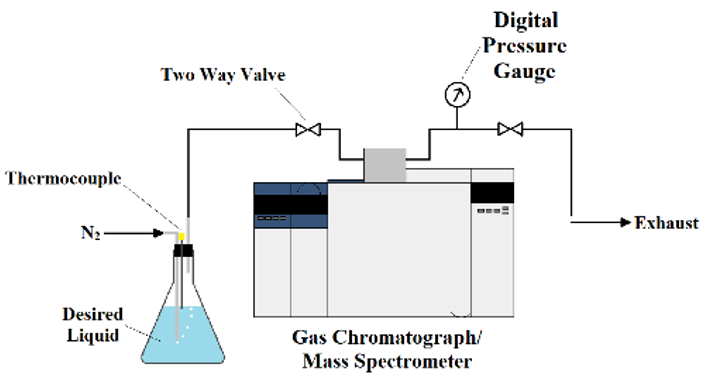
\includegraphics[width=\textwidth,keepaspectratio]{Bubbler_Setup.png}
	\caption[Flow diagram for bubble calibration system used for liquid materials]{Flow diagram for bubble calibration system used for liquid materials (acetone, ethanol, methanol, and water)}
	\label{fig:Bubbler}
\end{figure}
Nitrogen, acting as a carrier gas, was bubbled at the bottom of a liquid bath which after reaching the liquid surface transport vapor molecules through a heated gas line and into the GC/MSD sample loop. The concentration of the vapor injected into the GC/MSD was calculated from a liquid-vapor pressure correlation provided by DIPPR\textsuperscript{\textregistered}.

\begin{equation}
\label{eq:liquid_vapor_pressure_correlation}
P_{vap} =e^{A+\frac{B}{T}+C~\ln{T}+D~T^{E}}
\end{equation}
In this correlation, $P_{vap}$ is the vapor pressure calculated from the temperature of the liquid bath, $T$, with the coefficients ($A$, $B$, $C$, $D$, $E$) specific to the liquid material. Table~\ref{tab:Liquid Calibrate_Table} lists all coefficients for each calibrated liquid, including the uncertainty of their respective correlations, $u_{corr}$. 

\begin{table}[!]
\caption{Liquid Vapor Pressure Correlation Coefficients for Various Calibrated Liquids}
\label{tab:Liquid Calibrate_Table}
\centering
	\footnotesize
	\begin{tabular}{lcccccc}
			\hline
%\\[0.0005cm]
\textbf{Liquid Material} &\textbf{A}& \textbf{B}& \textbf{C}&\textbf{D}&\textbf{E}&\textbf{Uncertainty(\%)}\\
\hline
\\[0.001cm]
Acetone	&	69.006	&	-5599.6	&	-7.0985	&	6.2237E-6	& 	2.00	&  3.00\\
Ethanol	&	73.304	&	-7122.3	&	-7.1424	&	2.8853E-6	& 	2.00	&  1.00\\
Methanol	&	82.718	&	-6904.5	&	-8.8622	&	7.4664E-6	& 	2.00	&  3.00\\
Water		&	73.649	&	-7258.2	&	-7.3037	&	4.1653E-6	& 	2.00	&  0.20\\
%\\[0.01cm]
\hline
\end{tabular}
\end{table}

The concentration range of each calibrated liquid typically spanned between 2~\% and 50~\%. Liquid bath temperatures were controlled using a heating plate positioned underneath the insulated bubbler. The temperature of the bath, $T_{b}$, was measured using a K-type thermocouple placed at the liquid bath's surface. The liquid bath temperature measurements were sampled at \SI{2.0}{\hertz} for \SI{50}{s} simultaneously with pressure and temperature measurements of the GC/MSD sample loop. Liquid-vapor calibrations were conducted once the bath a steady-state temperature (approximately 1 hour) and the Nitrogen/vapor gas mixture has swept through the GC/MSD sample loop. Upon injection into the GC/MSD, pressure and temperature measurements of the sample loop are made as previously describe in Appendix~\ref{ssec:Total Moles Injected into the GC/MSD for Calibation}.

The uncertainty of the concentration determined using Eqn.~\ref{eq:liquid_vapor_concentration} was estimated using the law of propagation of uncertainty:
\begin{equation}
\label{eq:vapor_concentration_uncertainty}
u_{\scriptscriptstyle C_{vap}} = \sqrt{{\left( \frac{\partial C_{vap}}{\partial P}\,u_{\scriptscriptstyle P} \right) }^2+{\left(\frac{\partial C_{vap}}{\partial P_{vap}}\,u_{\scriptscriptstyle P_{vap}}\right)}^2}
\end{equation}

The uncertainty of the pressure measured upon injected was calculated from Eqn.~\ref{eq:pressure_uncertainty}. The uncertainty of the vapor pressure was found by combining the propagated error of liquid bath temperauture and the uncertainty in the correlation via quadrature:

\begin{equation}
\label{eq:vapor_concentration_uncertainty}
u_{\scriptscriptstyle P_{vap}} = \sqrt{{\left(\frac{\partial P_{vap}}{\partial T_{B}}\,u_{\scriptscriptstyle T_{B}} \right)}^2+{u_{corr}}^2}
\end{equation} 

The Type A evaluation of uncertainty of the liquid bath temperautre readings was determined from the standard error of the temperature, $s_{T_{B}}$ readings from the sampling period. The Type B evaluation of uncertainty for the liquid bath temperature was defined as the bias error source (\SI{1.5}{\degree C}) in the thermocouple, $u_{inst}$. The combined uncertainty liquid bath temperature was determined via quadrature:

\begin{equation}
\label{eq:temp_bath_uncertainty}
u_{\scriptscriptstyle T_{B}} = \sqrt{u_{\rm \scriptscriptstyle inst.}^2 + s_{\scriptscriptstyle T_{B}}^2}
\end{equation}
\pagebreak

\section{Uncertainty Analysis of the Soot Mass Fraction} \label{sec:Uncertainty_Soot_Frac}
\addcontentsline{toc}{section}{Appendix E: Uncertainty Analysis of the Soot Mass Fraction}
The local soot mass fraction measurements, $M_{s}$ made at various heights above the fuel surface in pool fires of different fuels were calculated through a combination of Eqns.~\ref{eq:soot_mass_frac}, \ref{eq:total_mass}, and \ref{eq:gas_density}:
\begin{equation}\label{eq:overall_soot_mass_frac}
Y_{s}= \frac{m_{s}~V_{sl}}{\dot{V}~t~m_{tot}}\frac{T_{\infty}}{T_{g}}
\end{equation}
where $m_{s}$ is the mass of soot collected on the PTFE filter and gun cleaning patches, $\dot{V}$ is the volumetric flow rate measured by the mass flow controller, $V_{sl}$ is the volume of the sample loop, $m_{tot}$ is the total mass of the gas sample detected in the TCD and TIC chromatograms calculated from the summation of the product of the number of moles of a given species and their respective molar mass, $T_{\infty}/T_{g}$ is the ratio of the internal gas flow temperature readings of the mass flow controller to the temperature of the probe, and $t$ is the total sampling time. The uncertainty of the measured soot mass fraction was estimated using the law of propagation of uncertainty after determing the soot mass fraction:

\begin{equation}
\label{eq:soot_mass_frac_uncertainty}
u_{\scriptscriptstyle Y_{s}} = \sqrt{{\left(\frac{\partial Y_{s}}{\partial m_{s}}\,u_{\scriptscriptstyle m_{s}} \right)}^2+{\left(\frac{\partial Y_{s}}{\partial \dot{V} }\,u_{\scriptscriptstyle \dot{V}} \right)}^2+{\left(\frac{\partial Y_{s}}{\partial m_{tot}}\,u_{\scriptscriptstyle m_{tot}} \right)}^2+{\left(\frac{\partial Y_{s}}{\partial T_{\infty}}\,u_{\scriptscriptstyle T_{\infty}} \right)}^2+{\left(\frac{\partial Y_{s}}{\partial T_{g}}\,u_{\scriptscriptstyle T_{g}} \right)}^2}
\end{equation}
A coverage factor of 2 was applied to the combined uncertainty to produce a 95~\% confidence interval.

\subsection{Mass of Soot}
\label{ssec:Mass_of_Soot}

The mass of soot was measured from the difference in mass of a dried PTFE filter and dried gun cleaning patches immediately before and \SI{48}{hrs} after each test. The Type A evaluation of standard uncertainty of the mass of soot, $m_{s}$ was taken as the standard deviation, $s_{m_{s}}$, of the measurements sampled three times before and after each test. The Type B evaluation of uncertainty, $u_{inst}$, was determined from the instrumentation error sources of the scale and was found to be 1~\% of the reading. The combined uncertainty was found via quadrature:

\begin{equation}
\label{eq:soot_mass_uncertainty}
u_{\scriptscriptstyle m_{s}} = \sqrt{u_{\rm \scriptscriptstyle inst}^2 + s_{\scriptscriptstyle m_{s}}^2}
\end{equation}

\subsection{Mass Flow Controller Volumetric Flow Rate}
\label{ssec:Mass_Flow_Controller_Volumetric_Flow_Rate}

A mass flow controller was used to measure the volumetric flow rate, $\dot{V}$, within the gas sampling line. The Type A evaluation of standard uncertainty was taken as the standard deviation of the flow measurements sampled at \SI{2}{Hz} during the gas sampling period which varied from\SI{12}{min} to \SI{25}{min} depending on the sampling location within the fire. The Type B evaluation of standard uncertainty was determined from the calibration error, $u_{cal}$, and the precision error sources at calibration conditions, $u_{p}$, defined as \SI{2}{ml} and 0.8~\% of the reading + 0.2~\% of the full scale (\SI{2}{L/min}), respectively. The combined uncertainty was calculated via quadrature:

\begin{equation}
\label{eq:volumetric_flow_uncertainty}
u_{\scriptscriptstyle \dot{V}} = \sqrt{u_{\rm \scriptscriptstyle p}^2 + u_{\rm \scriptscriptstyle cal}^2 + s_{\scriptscriptstyle \dot{V}}^2}
\end{equation}

\subsection{Total Mass Identified}
\label{ssec:Total_Mass_Identified_into_GC/MSD}
The total mass detected in the TCD and TIC chromatograms, $m_{tot}$, was calculated from the summation of products of the number moles of a given species that were identified from the TCD and TIC chromatograms, $n_{i}$, and their respective molar mass, ${\textrm{MW}_{i}}$: 

\begin{equation}
\label{eq:total_mass_detected_uncertainty}
m_{tot}=\sum_{n=1}^{N} n_{i}{\textrm{MW}_{i}}
\end{equation}

The uncertainty in the total mass detected was calculated from the uncertainties of all identified species, defined in Section~\ref{ssec:Total Number of Moles Identified}, multiplied by their corresponding molar mass via quadrature:

\begin{equation}
\label{eq:total_mass_detected_uncertainty}
u_{\scriptscriptstyle m_{tot}}=\sqrt{{\sum_{n=1}^{N} (u_{\scriptscriptstyle n_{i}}{\textrm{MW}_{i}})^2}}
\end{equation}
where $N$ is the number of a species identified species in the TCD and TIC chromatograms. 

\subsection{Mass Flow Controller Internal Gas Flow Temperature Reading}
\label{ssec:MFC_Temp}

The mass flow controller provides an internal gas flow temperature reading that was recorded manually during the gas sampling process. The uncertainty of the temperature reading was determined from the Type B evaluation of standard uncertainty of the mass flow controller temperature measurement defined as 0.75~\% of the reading.

\subsection{The Effective Temperature of the Gas}
\label{ssec:Probe_Temp}

The uncertainty of the temperature measurements at the entrance of the probe is described in Appendix~\ref{sec:Uncertainty_Temperature_Measurements}.

\pagebreak

\section{Uncertainty Analysis of the Mixture Fraction}\label{sec:Uncertainty_Mix_Frac}
\addcontentsline{toc}{section}{Appendix F: Uncertainty of the Mixture Fraction}
The mixture fraction, $Z$, was determined from Eqn.~\ref{eq:Mixture_Fraction} based on carbon containing species. The uncertainty of the determined mixture fraction was estimated from the law of propagation of uncertainty using mass fractions of carbon containing species, $\bar{Y}_{i,c}$, and the parent fuel, $\bar{Y}_{f}$.
\begin{equation}
\label{eq:mixture_frac_uncertainty}
u_{\scriptscriptstyle Z}=\sqrt{{u_{\scriptscriptstyle \bar{Y}_{f}}}^2+{\sum_{i=1}^{N}{\left(\frac{\partial Z}{\partial \bar{Y}_{i,C}}\frac{u_{\scriptscriptstyle \bar{Y}_{i,C}}}{\textrm{MW}_{i}} \right)}^2}}
\end{equation}
The uncertainty of the mass fractions of carbon containing species is discussed in Appendix~\ref{ssec:Uncertainty of Mass Fractions}. 

\pagebreak

\section{Uncertainty Analysis of the $Z^{*}$}\label{sec:Uncertainty_Z_star}
\addcontentsline{toc}{section}{Appendix H: Uncertainty Analysis of the $Z^{*}$}
$Z^{*}$ was calculated from Eqn.~\ref{eq:Z_Star} where the gravitational constant and temperature, specific heat, and density of the ambient air were treated as constants. The uncertainty of $Z^{*}$ was calculated from the law of propagation of uncertainty, which incorporated the uncertainties of the heat release rate, $\dot{Q}$, and the mean flame height, $H$. 
\begin{equation}
\label{eq:heat_release_rate_uncertainty}
u_{\scriptscriptstyle Z^{*}} = \sqrt{{\left(\frac{\partial Z^{*}}{\partial \dot{Q}}\,u_{\scriptscriptstyle \dot{Q}} \right)}^2+{\left(\frac{\partial Z^{*}}{\partial H}\,u_{\scriptscriptstyle H} \right)}^2}
\end{equation}
The uncertainty of the heat release rate and mean flame height is described in Appendix~\ref{sec:Uncertainty_Pool_Fire_Parameters}. 

\pagebreak

\section{Figures of Averaged Volume Fractions of Centerline Measurements as a Function of $Z^{*}$ for Methanol, Ethanol, and Acetone Fires}\label{sec:Vol_Frac_Figs}
\addcontentsline{toc}{section}{Appendix H: Figures of Averaged Volume Fractions of Centerline Measurements as a Function of $Z^{*}$ for Methanol, Ethanol, and Acetone Fires}

\subsection{Methanol}
\label{ssec:Methanol_ALL_Vol_Frac}
\begin{figure}[!h]
	\centering
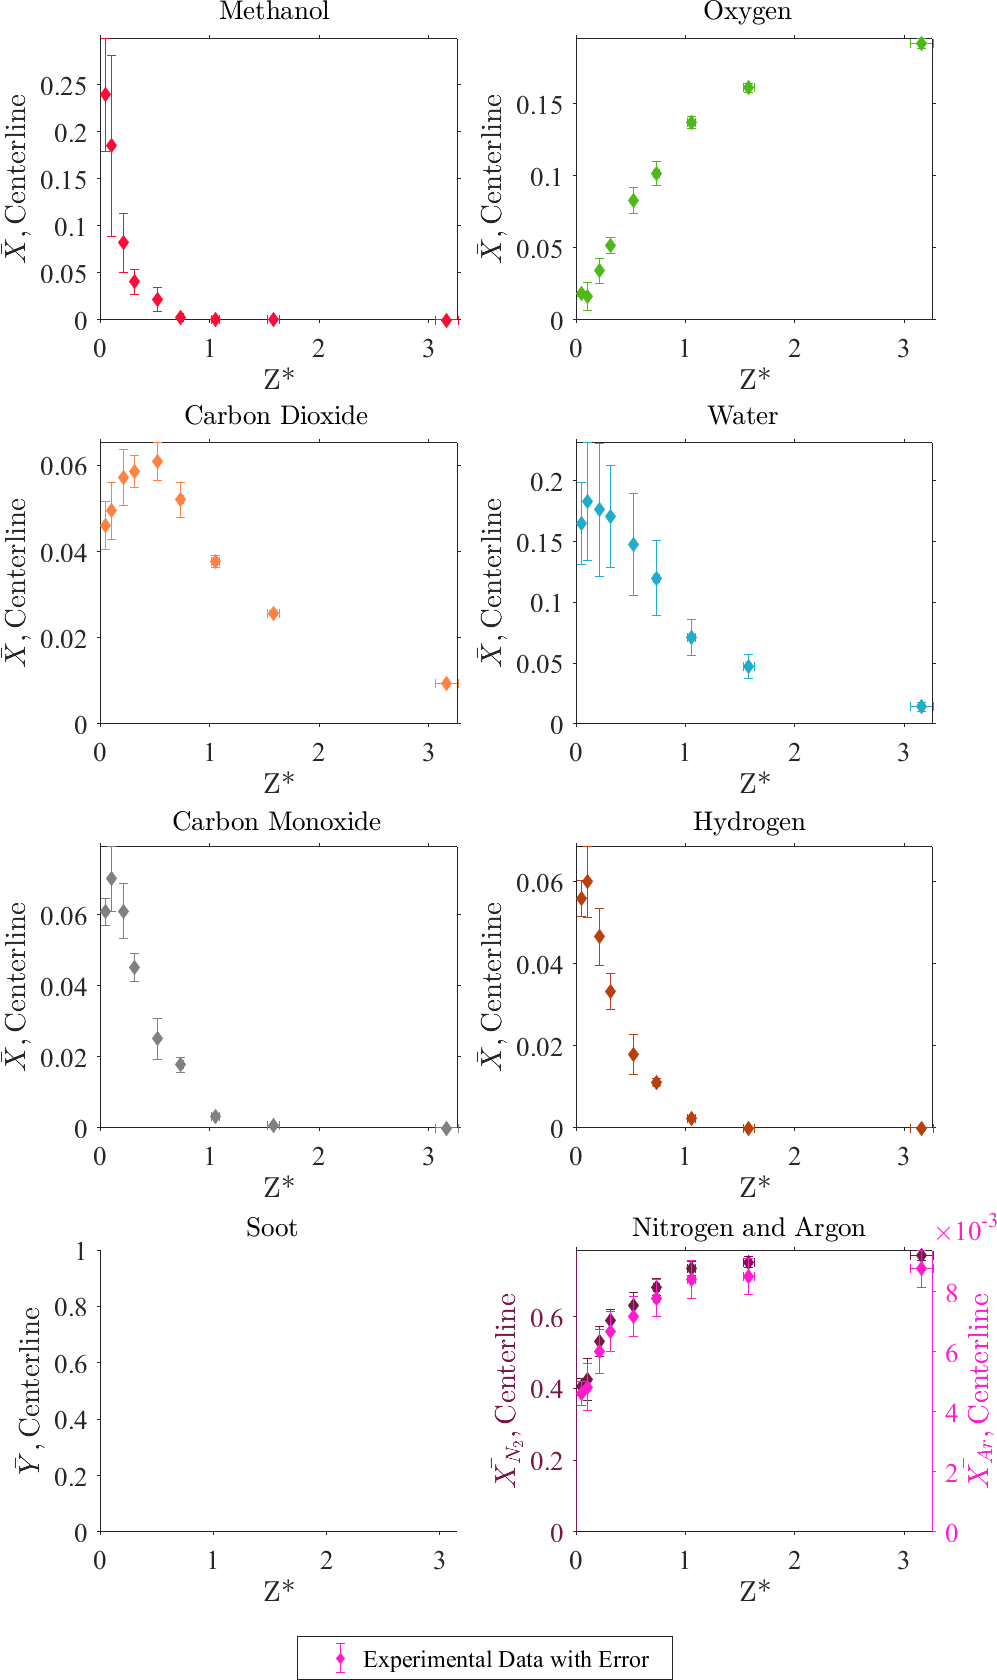
\includegraphics[width=10.0cm,keepaspectratio]{Methanol_MOL_FRAC_Plot.png}
	\caption[Plot of volume fractions, with error, of major species identified in the methanol pool fire centerline as function of $Z^{*}$]{Plot of volume fractions of major species identified in the methanol pool fire centerline as function of $Z^{*}$}
	\label{fig:Methanol_VOL_Frac_Major}
\end{figure}
\pagebreak

\begin{figure}[!h]
	\centering
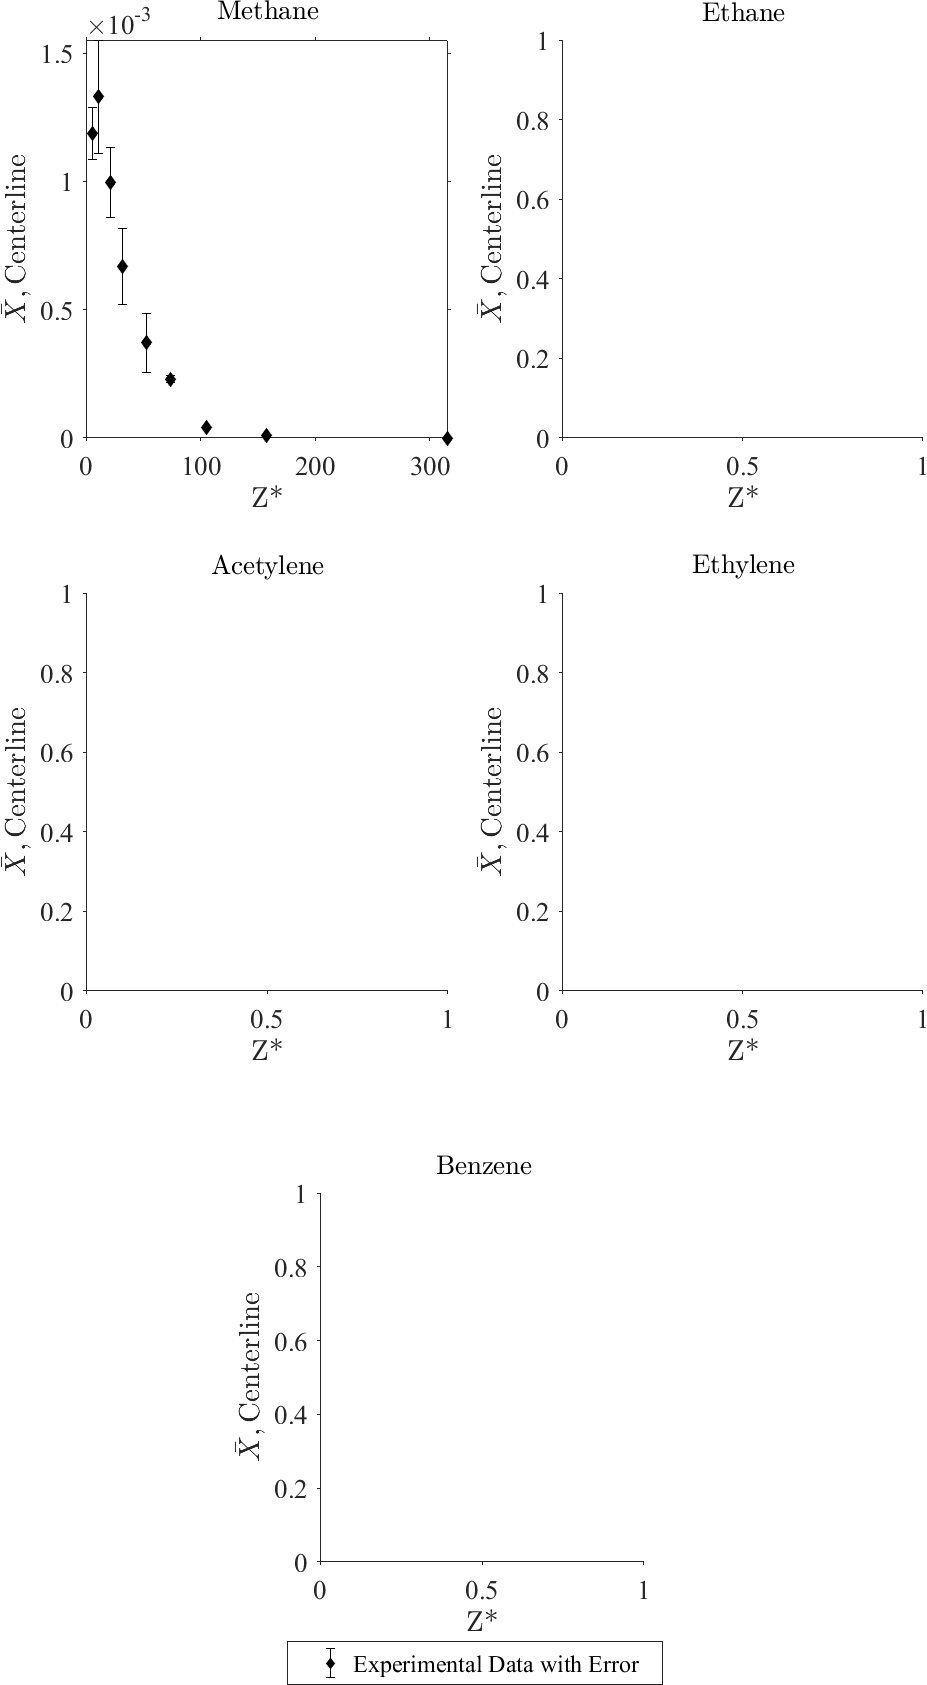
\includegraphics[width=10.0cm,keepaspectratio]{Methanol_Inter_MOL_FRAC_Plot.png}
	\caption[Plot of volume fractions, with error, of intermediate species identified in the methanol pool fire centerline as function of $Z^{*}$]{Plot of volume fractions of intermediate species identified in the methanol pool fire centerline as function of $Z^{*}$}
	\label{fig:Methanol_VOL_Frac_Inter}
\end{figure}
\pagebreak

\subsection{Ethanol}
\label{ssec:Ethanol_ALL_Vol_Frac}

\begin{figure}[!h]
	\centering
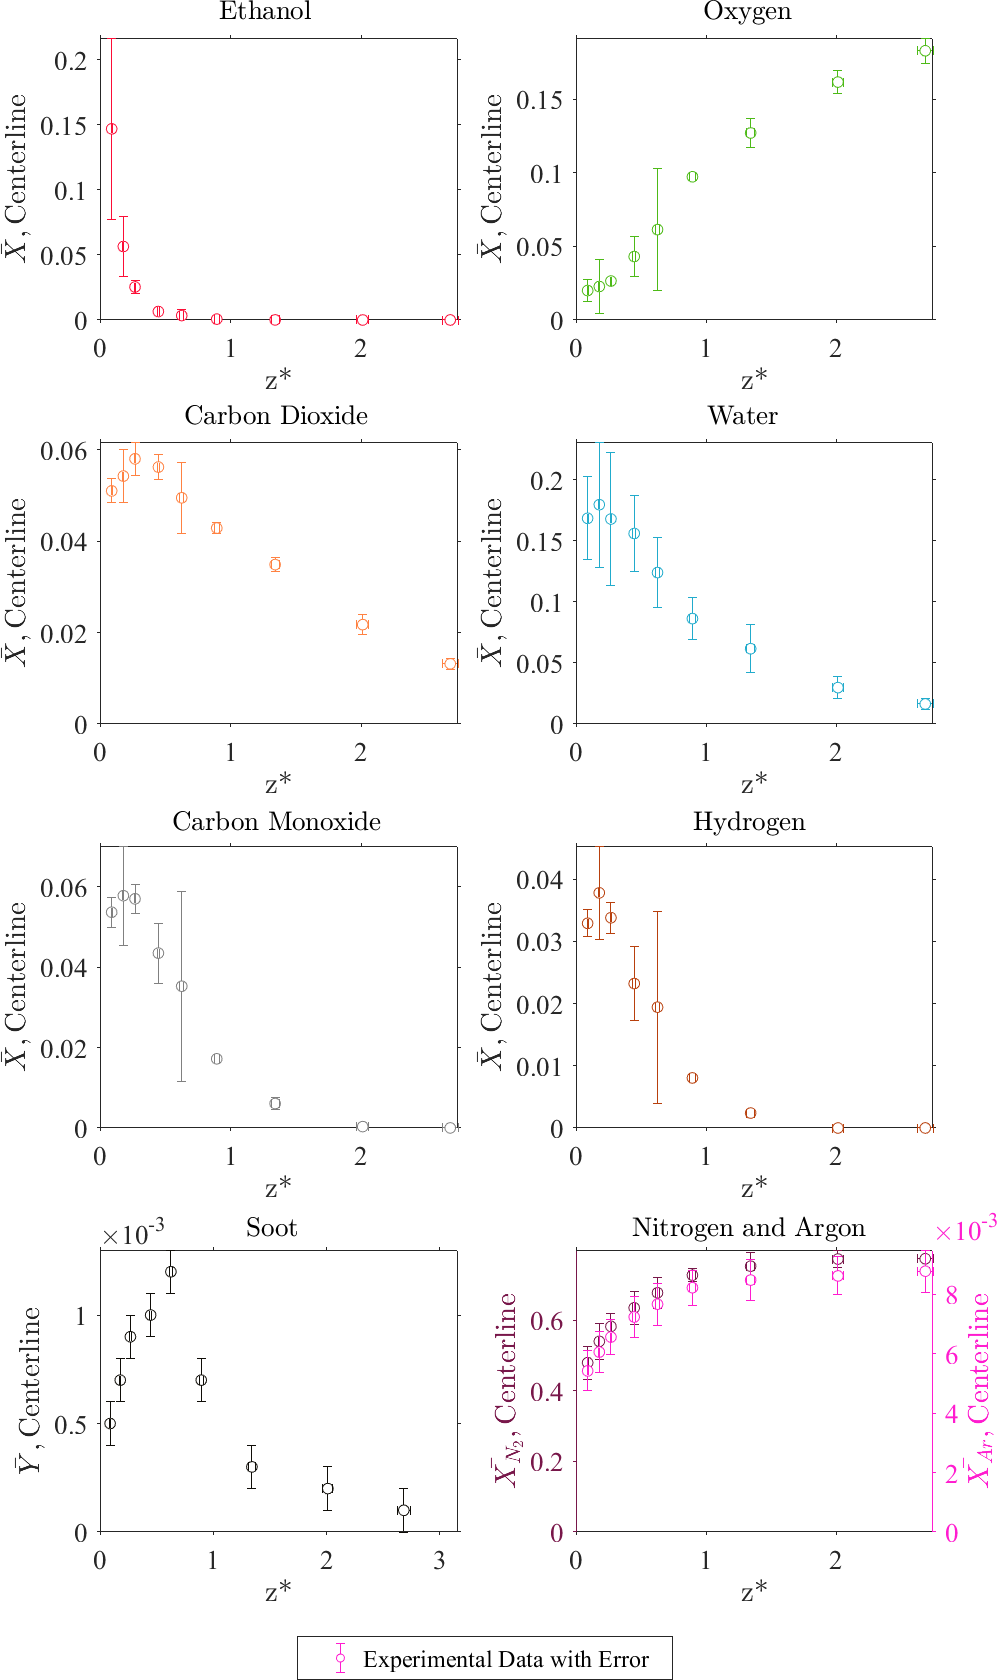
\includegraphics[width=10.5cm,keepaspectratio]{Ethanol_MOL_FRAC_Plot.png}
	\caption[Plot of volume fractions, with error, of major species identified in the ethanol pool fire centerline as function of $Z^{*}$]{Plot of volume fractions of major species identified in the ethanol pool fire centerline as function of $Z^{*}$}
	\label{fig:Methanol_VOL_Frac_Major}
\end{figure}
\pagebreak

\begin{figure}[!h]
	\centering
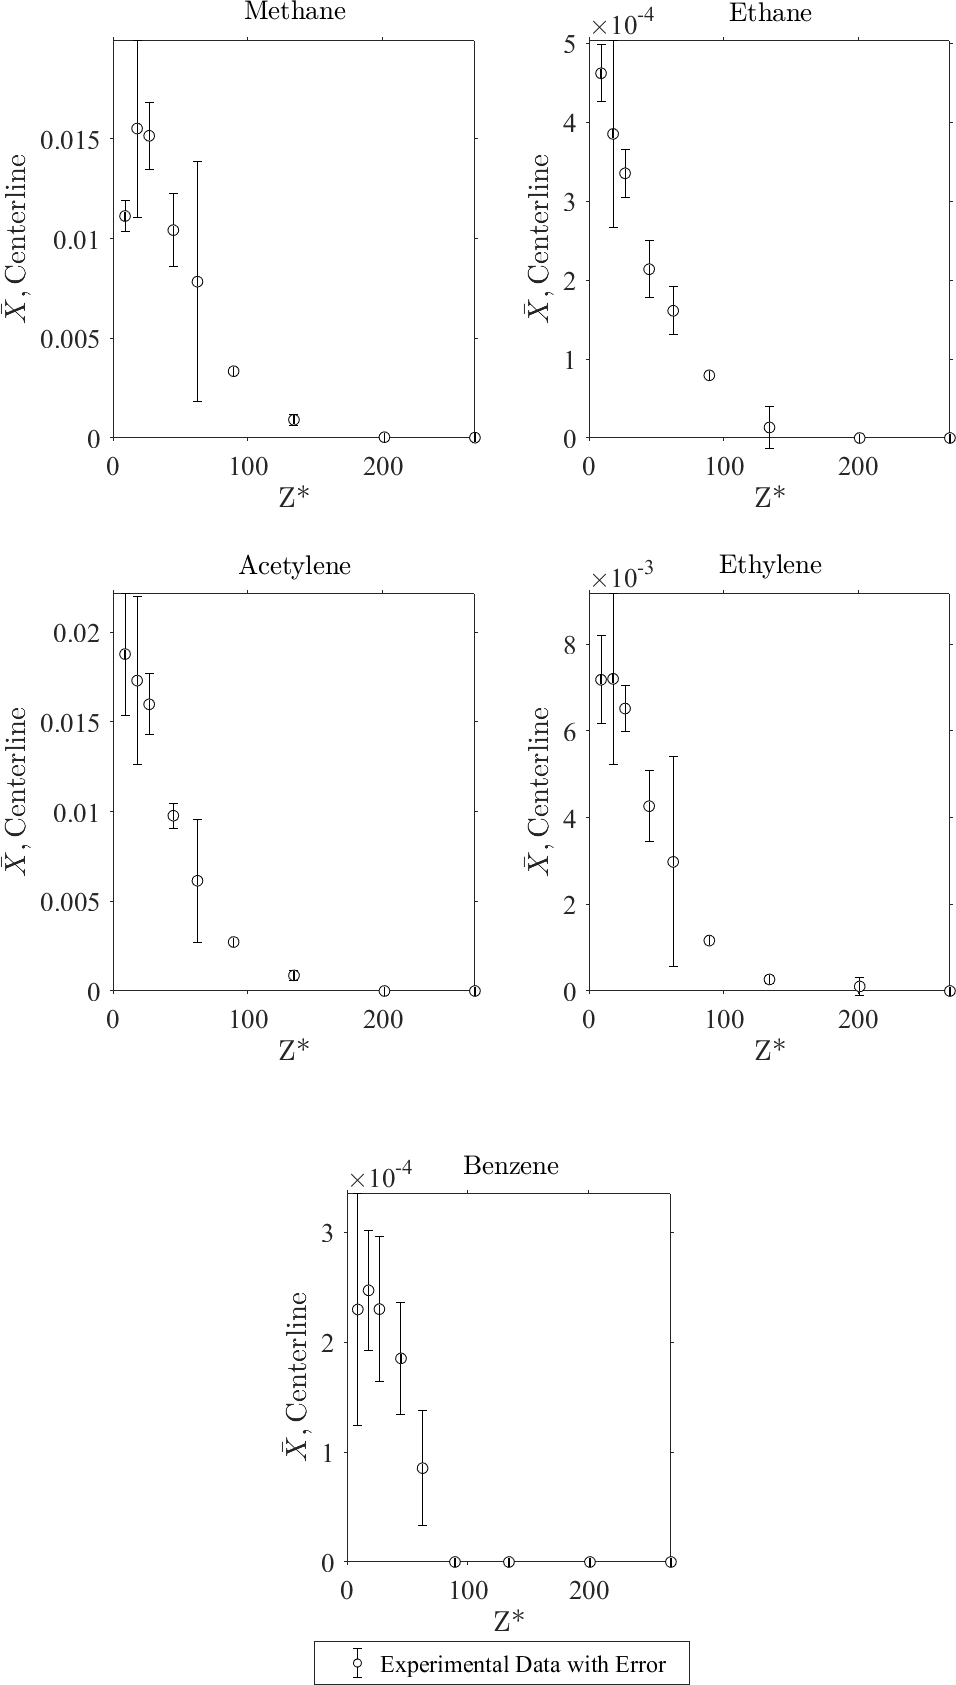
\includegraphics[width=10.5cm,keepaspectratio]{Ethanol_Inter_MOL_FRAC_Plot.png}
	\caption[Plot of volume fractions, with error, of intermediate species identified in the ethanol pool fire centerline as function of $Z^{*}$]{Plot of volume fractions of intermediate species identified in the ethanol pool fire centerline as function of $Z^{*}$}
	\label{fig:Methanol_VOL_Frac_Inter}
\end{figure}


\pagebreak
\subsection{Acetone}
\label{ssec:Acetonel_ALL_Vol_Frac}

\begin{figure}[!h]
	\centering
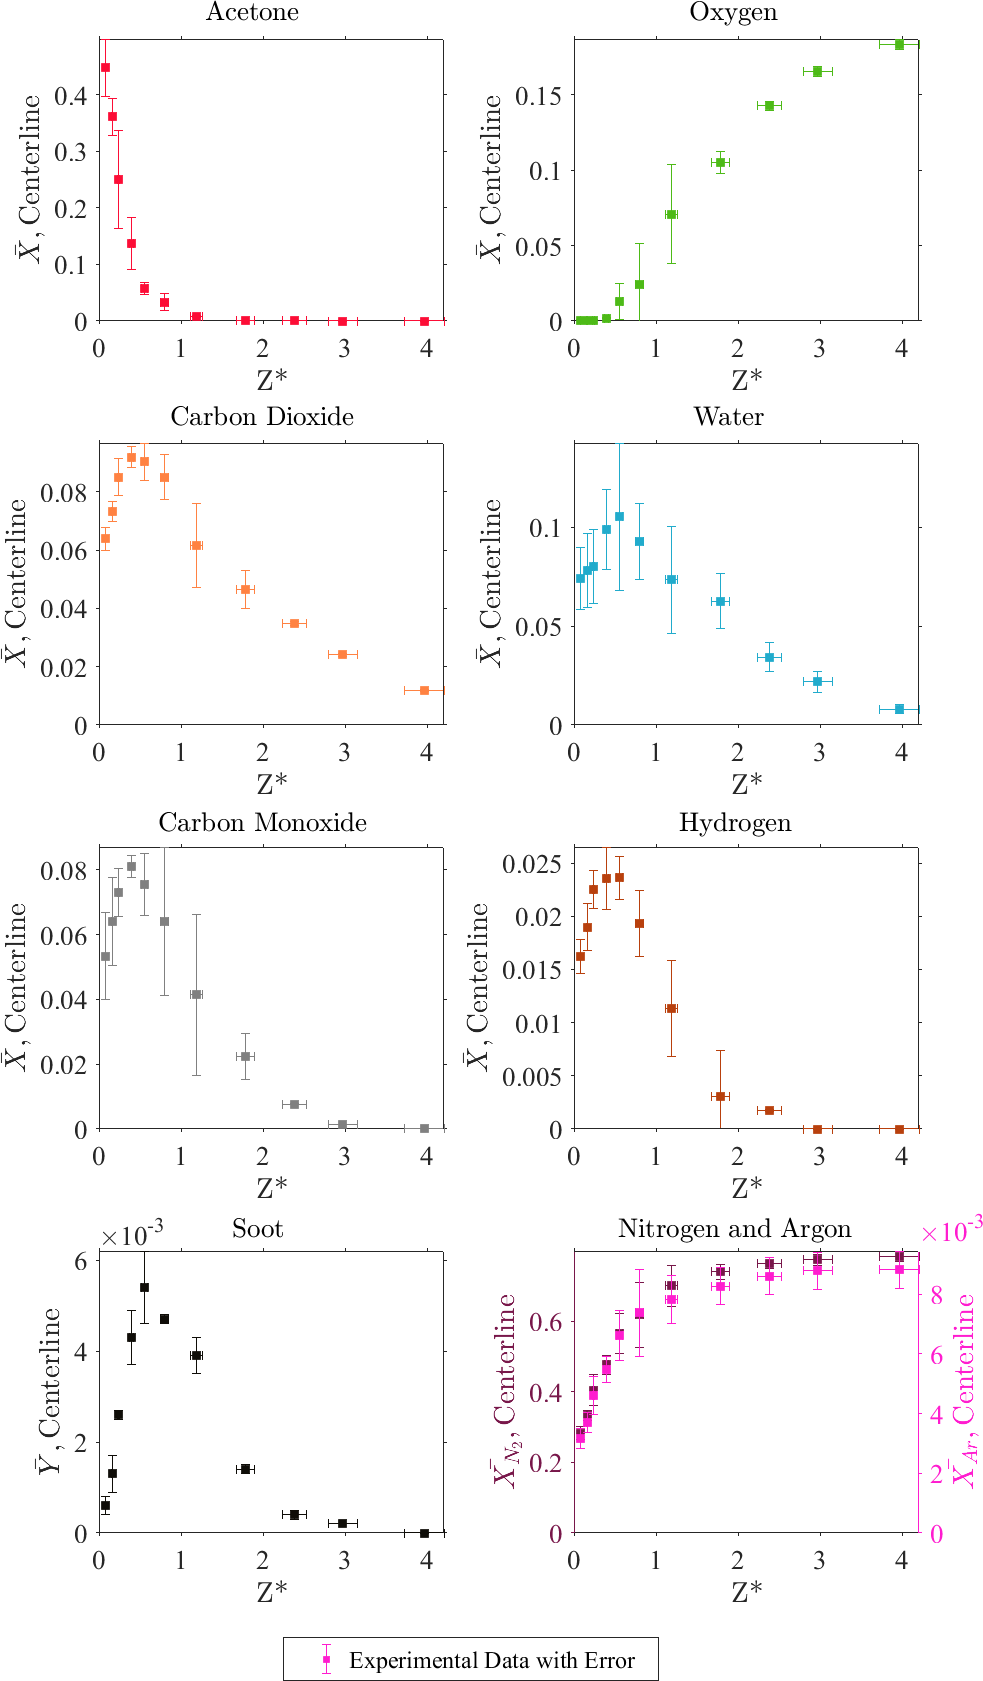
\includegraphics[width=10.0cm,keepaspectratio]{Acetone_MOL_FRAC_Plot.png}
	\caption[Plot of volume fractions, with error, of major species identified in the acetone pool fire centerline as function of $Z^{*}$]{Plot of volume fractions of major species identified in the acetonel pool fire centerline as function of $Z^{*}$}
	\label{fig:Methanol_VOL_Frac_Major}
\end{figure}

\begin{figure}[!h]
	\centering
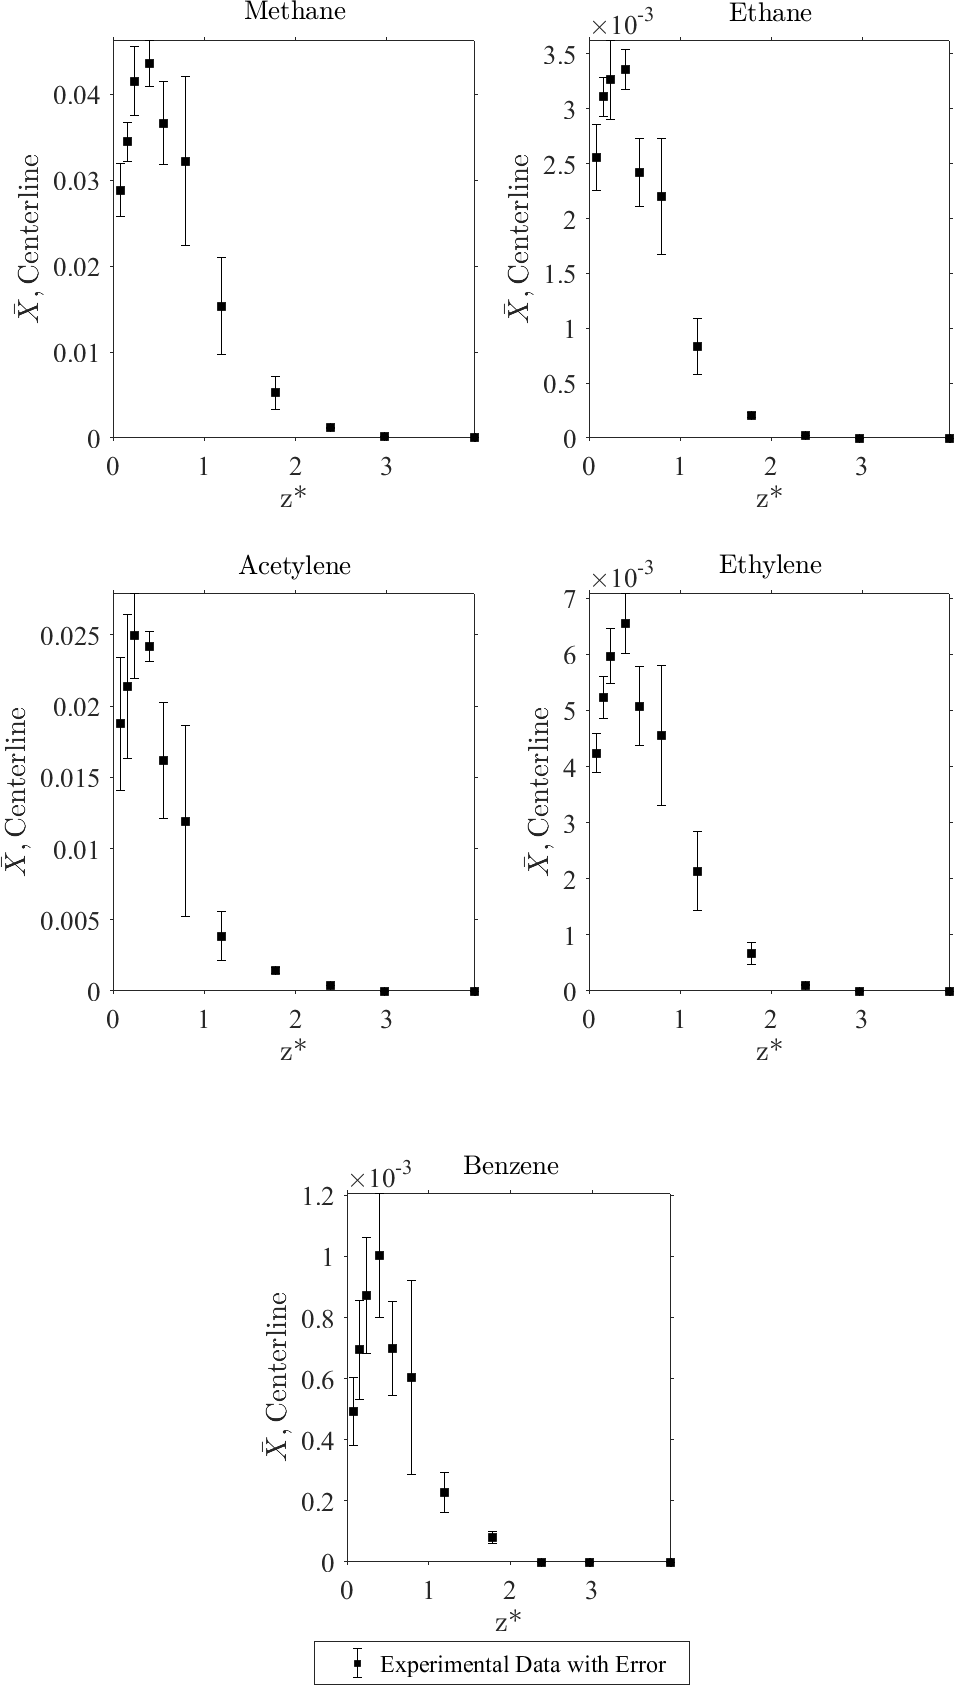
\includegraphics[width=10.0cm,keepaspectratio]{Acetone_Inter_MOL_FRAC_Plot.png}
	\caption[Plot of volume fractions, with error, of intermediate species identified in the acetone pool fire centerline as function of $Z^{*}$]{Plot of volume fractions of intermediate species identified in the acetone pool fire centerline as function of $Z^{*}$}
	\label{fig:Methanol_VOL_Frac_Inter}
\end{figure}

\pagebreak

\section{Figures of Averaged Mass Fractions of Centerline Measurements as a Function of Mixture Fractions for Methanol, Ethanol, and Acetone Fires}\label{sec:Mix_Frac_Figs}
\addcontentsline{toc}{section}{Appendix I: Figures of Averaged Mass Fractions of Centerline Measurements as a Function of Mixture Fractions for Methanol, Ethanol, and Acetone Fires}

\subsection{Methanol}
\label{ssec:Methanol_ALL_Mix_Frac}

\begin{figure}[!h]
	\centering
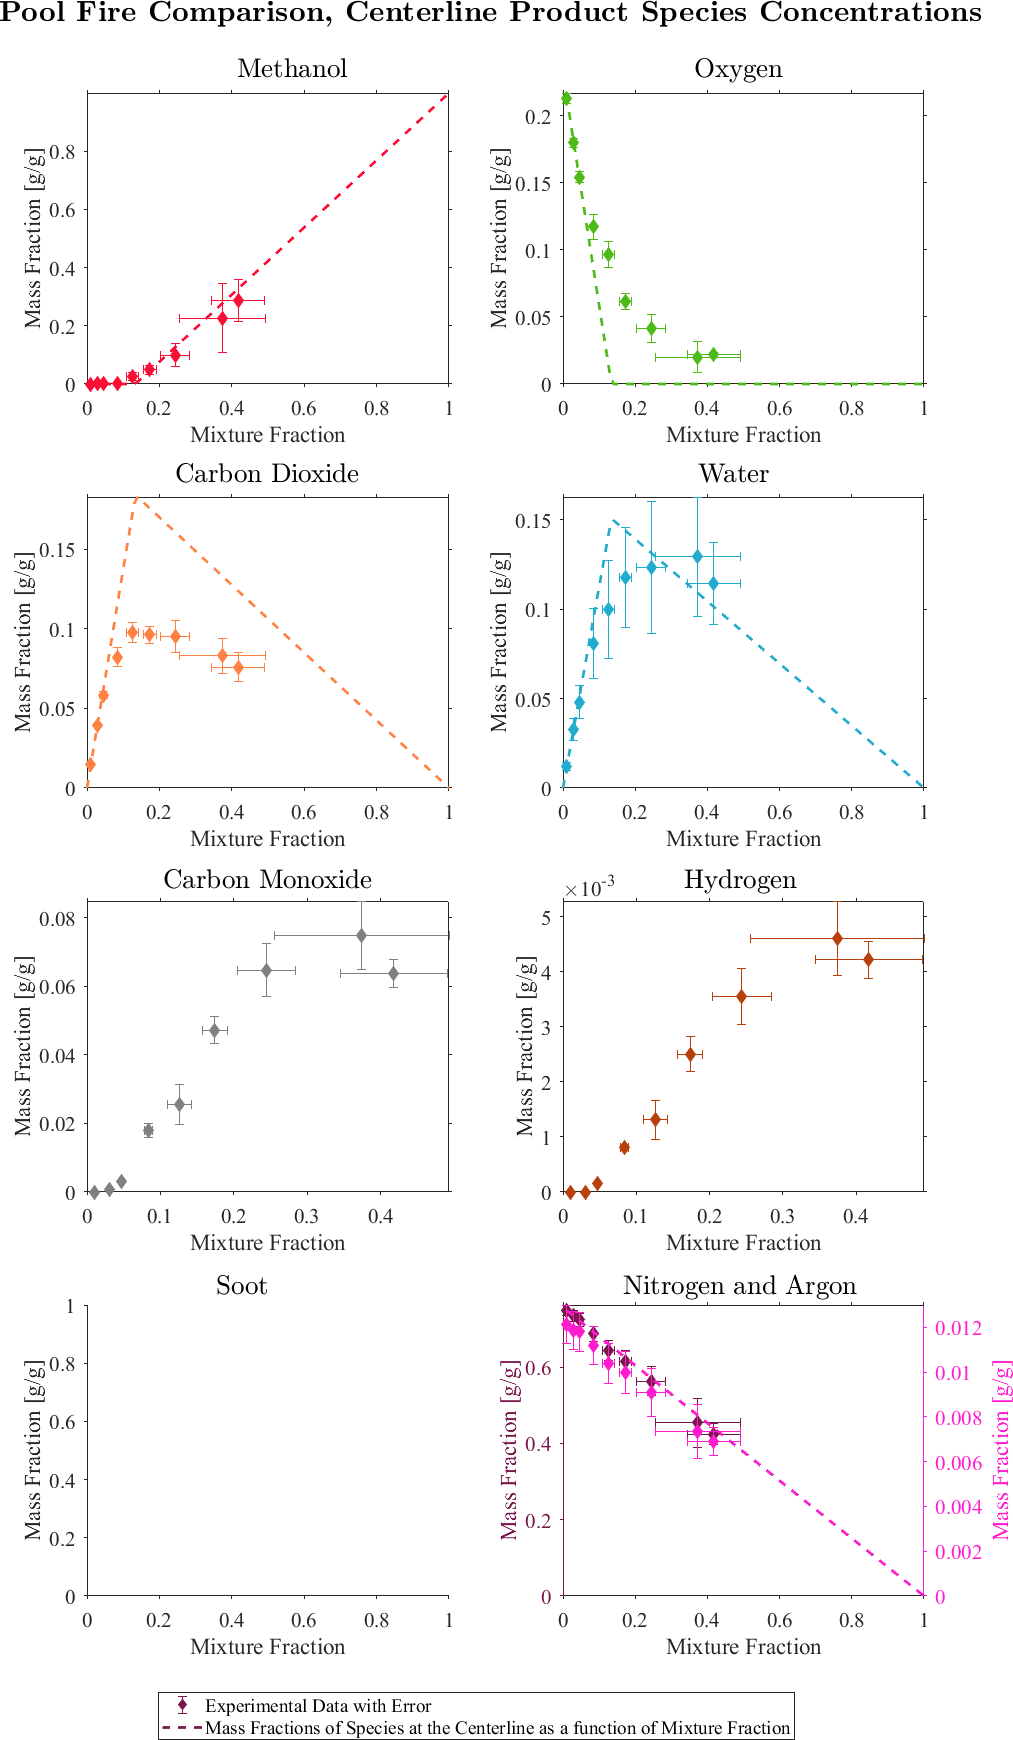
\includegraphics[width=10.0cm,keepaspectratio]{Methanol_Mixture_Fraction_Major_Plot.png}
	\caption[Plot of mass fractions, with error, of major species identified in the methanol pool fire centerline as function of mixture fraction]{Plot of mass fractions, with error, of major species identified in the methanol pool fire centerline as function of mixture fraction}
	\label{fig:Methanol_MIX_Frac_Major}
\end{figure}

\pagebreak

\subsection{Ethanol}
\label{ssec:Ethanol_ALL_Mix_Frac}
\begin{figure}[h!]
	\centering
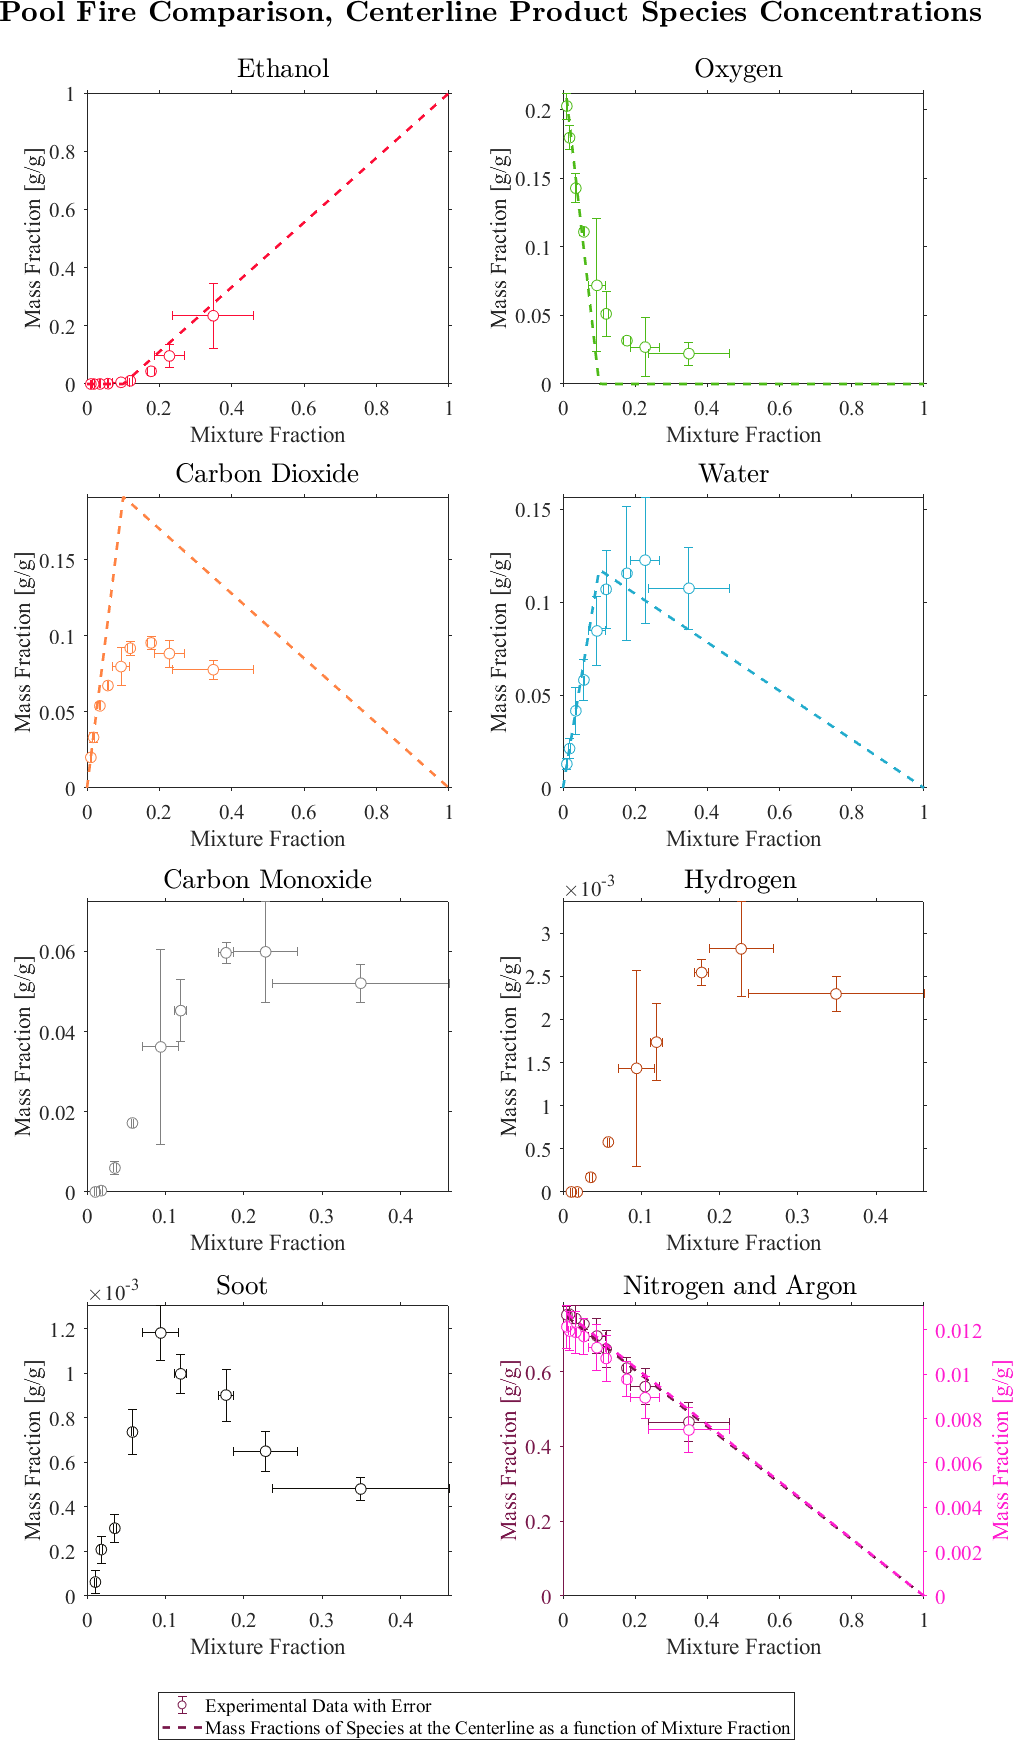
\includegraphics[width=10.0cm,keepaspectratio]{Ethanol_Mixture_Fraction_Major_Plot.png}
	\caption[Plot of mass fractions, with error, of major species identified in the ethanol pool fire centerline as function of mixture fraction]{Plot of mass fractions, with error, of major species identified in the ethanol pool fire centerline as function of mixture fraction}
	\label{fig:Ethanol_MIX_Frac_Major}
\end{figure}

\pagebreak

\subsection{Acetone}
\label{ssec:Acetone_ALL_Mix_Frac}
\begin{figure}[!h]
	\centering
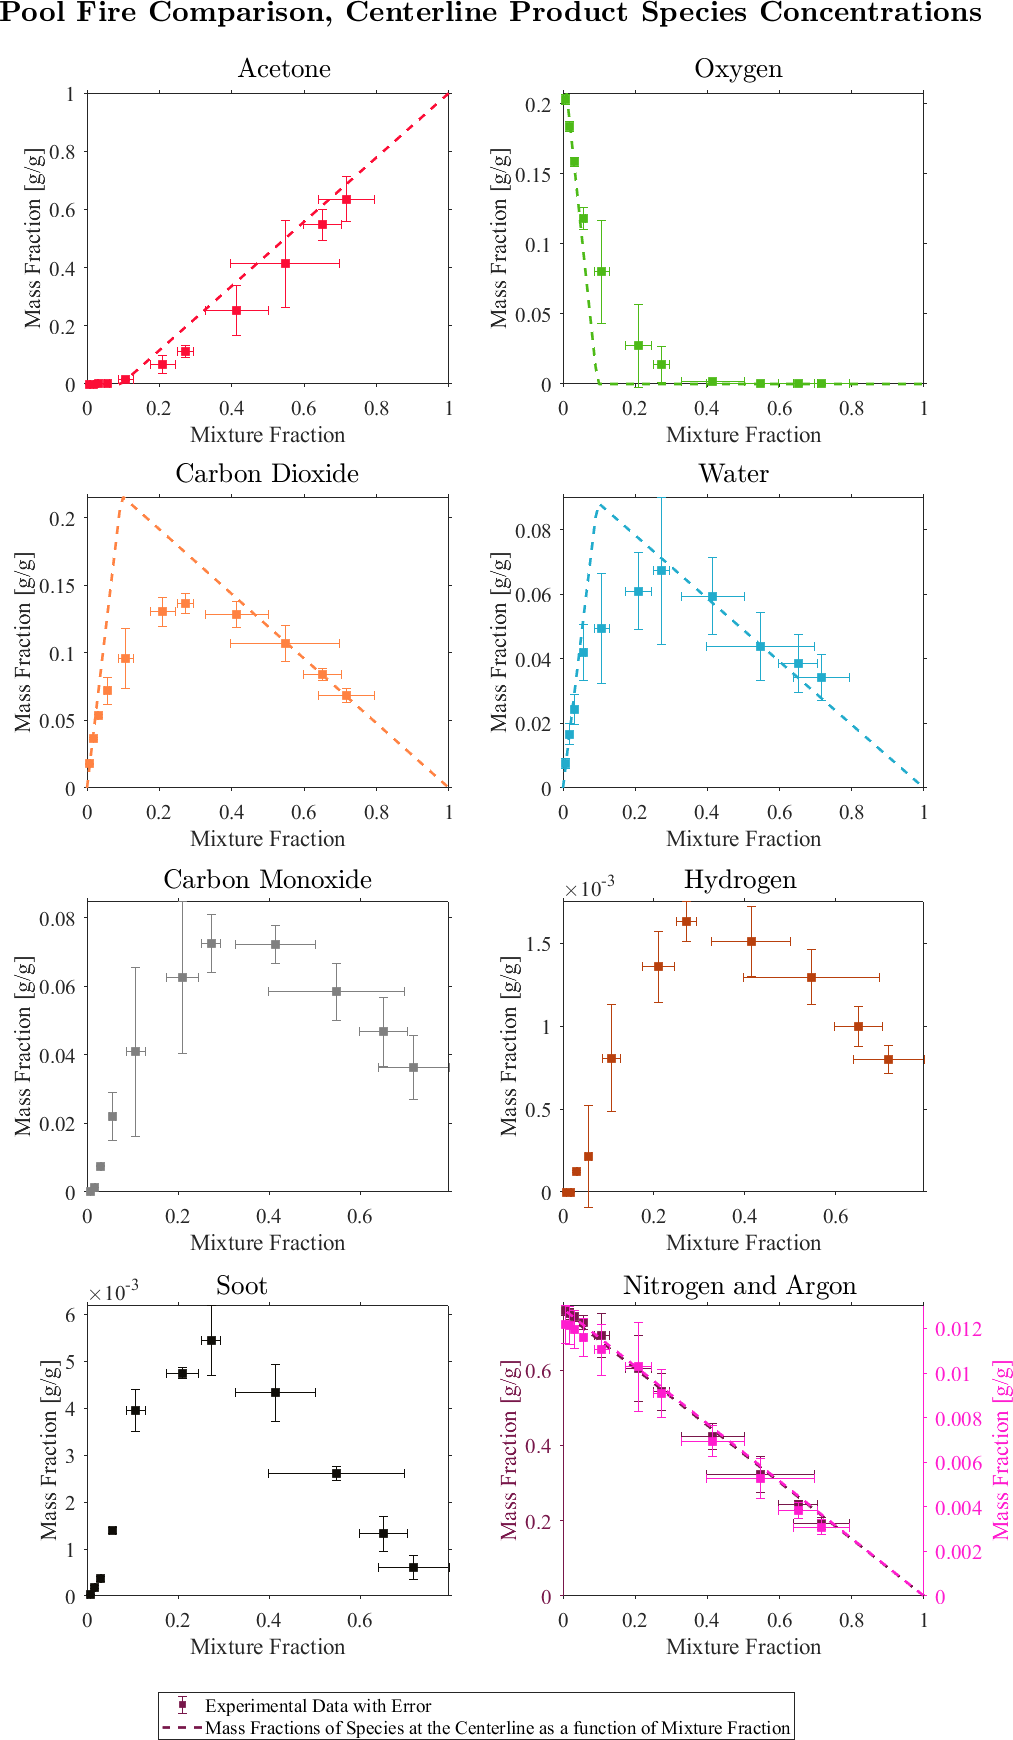
\includegraphics[width=10.0cm,keepaspectratio]{Acetone_Mixture_Fraction_Major_Plot.png}
	\caption[Plot of mass fractions, with error, of major species identified in the acetone pool fire centerline as function of mixture fraction]{Plot of mass fractions, with error, of major species identified in the acetone pool fire centerline as function of mixture fraction}
	\label{fig:Acetone_MIX_Frac_Major}
\end{figure}

\pagebreak

\section{Uncertainty Analysis of the Verification Scheme}\label{sec:Uncertainty_Ver_Scheme}
\addcontentsline{toc}{section}{Appendix J: Uncertainty of the Verification Scheme}
\subsection{Ratio of moles identified to moles injected }
\label{ssec:mole ratio}
The uncertainty of the ratio of the total number of moles identified by the TCD and MSD, $n_{tot}$, to the number of moles injected into the GC/MSD, $n_{inj}$, was calculated using the law of propagation of uncertainty and shown in the equation below:
\begin{equation}
\label{eq:mol_ratio_uncertainty}
u_{\scriptscriptstyle n_{tot}/n_{inj}} = \sqrt{\left(\frac{u_{\scriptscriptstyle n_{tot}}}{n_{inj}}\right)^2 + \left(\frac{-n_{tot}~u_{\scriptscriptstyle n_{inj}}}{{n_{inj}^2}}\right)^2}
\end{equation}
The uncertainty of the total number of moles identified, $n_{tot}$, is described in Section~\ref{ssec:Total Number of Moles Identified}. The uncertainty of the number of moles injected into the GC/MSD, $n_{inj}$, is described in Section~\ref{ssec:Total Moles Injected into the GC/MSD for Calibation}.

\subsection{Carbon to Hydrogen Ratio}
\label{ssec:C2H_ratio}
The carbon to hydrogen ratio was calculated using Eqn.~\ref{eq:c2h_ratio} using the mass fraction of any quantified gas species that contained either carbon, $\bar{Y}_{i,C}$, or hydrogen, $\bar{Y}_{i,H}$.
\begin{equation}
\label{eq:c2h_uncertainty}
u_{\scriptscriptstyle {C}/{H}} = \sqrt{{\sum\left(\frac{\partial ({C}/{H})}{\partial \bar{Y}_{i,C}}\,u_{\scriptscriptstyle \bar{Y}_{i,C}}~{\frac{\textrm{MW}_{C}}{\textrm{MW}_{i,C}}} \right)}^2+{\sum\left(\frac{\partial ({C}/{H})}{\partial Y_{i,H}}\,u_{\scriptscriptstyle \bar{Y}_{i,H}}{\frac{\textrm{MW}_{H}}{\textrm{MW}_{i,H}}} \right)}^2}
\end{equation}
The uncertainty of the mass fractions of carbon and hydrogen containing species is described in Appendix~\ref{ssec:Uncertainty of Mass Fractions}.

\subsection{Stoichiometric Combustion Ratio}
\label{ssec:Pro_ratio}
The stoichiometric combustion ratio, $\text{SCR}$, was calculated from a ratio of volume fractions of combustion products, $\bar{X}_{i}$, identified by the TCD and TIC chromatograms. The uncertainty of $\text{SCR}$ was determined from the law of propagation of uncertainty:
\begin{equation}
\label{eq:c2h_ratio_uncertainty}
u_{\scriptscriptstyle \text{SCR}} = \sqrt{{\sum\left(\frac{\partial \text{SCR}}{\partial \bar{X}_{i}}\,u_{\scriptscriptstyle \bar{X}_{i}}\right)}^2}
\end{equation}
The uncertainty of the volume fractions is described in Appendix~\ref{sec:UncertaintyMoleFrac}.

\subsection{Inert Ratio}
\label{ssec:Inert_ratio}
The inert ratio was calculated from the ratio the Nitrogen and Argon volume fractions, $\bar{X}_{N_2}$ and $\bar{X}_{Ar}$, identified by the TCD and TIC chromatograms. The uncertainty of inert ratio was determined from the law of propagation of uncertainty:
\begin{equation}
\label{eq:inert_ratio_uncertainty}
u_{\scriptscriptstyle \bar{X}_{N_2}/\bar{X}_{Ar}} = \sqrt{{\left(\frac{u_{\scriptscriptstyle \bar{X}_{N_2}}}{\bar{X}_{Ar}}\right)}^2+{\left(\frac{-\bar{X}_{N_2}u_{\scriptscriptstyle \bar{X}_{Ar}}}{\bar{X}_{Ar}}\right)}^2}
\end{equation}
The uncertainty of the volume fractions is described in Appendix~\ref{sec:UncertaintyMoleFrac}.

\pagebreak

\section{Derivations of the Stoichiometric Combustion Ratio for Methanol, Ethanol, and Acetone Fires}\label{sec:SCR_Derv}
\addcontentsline{toc}{section}{Appendix K : Derivations of the Stoichiometric Combustion Ratio for Methanol, Ethanol, and Acetone Fires}
\subsection{Methanol}
\label{ssec:Methanol_SCR}
The combustion of methanol was determined from the gas species identified by the GC/MSD and is shown in the reaction below.
\begin{align*}
CH_{3}OH+&a~(O_{2}+3.76~N_{2}+0.0445~Ar)\\
&\rightarrow b~CH_{3}OH+c~O_{2}+ d~CO_{2}+e~H_{2}O\\
&~~~~+f~H_{2}+ g~CO+h~CH_{4}\\
&~~~~+i~(3.76~N_{2}+0.0445~Ar) \numberthis \label{eq:Methanol_rxn}
\end{align*}
Balancing the hydrogen atoms produces the following equation:
\begin{equation}
\label{eq:Methanol_H_Balance_1}
4b+2e+2f+4h=4
\end{equation}
This equation can be rewritten as:
\begin{equation}
\label{eq:Methanol_H_Balance_2}
-\frac{1}{2}\left(e+f\right)=b+h-1
\end{equation}
Balancing the carbon atoms results in:
\begin{equation}
\label{eq:Methanol_C_Balance_1}
b+d+g+h=1
\end{equation}
Eqn.~\ref{eq:Methanol_H_Balance_2} can then be substituted into Eqn.~\ref{eq:Methanol_C_Balance_1}, resulting in
\begin{equation}
\label{eq:Methanol_C_Balance_2}
d+g-\frac{1}{2}\left(e+f\right)=0
\end{equation}
or 
\begin{equation}
\label{eq:Methanol_SCR}
\frac{e+f}{d+g}=2
\end{equation}
When simplified, Eqn.~\ref{eq:Methanol_SCR} is shown to equal a constant value, which is defined as the $\text{SCR}$ of methanol.
\begin{equation}\label{eq:prod_ratio_methanol}
 \text{SCR}_{methanol}=\frac{\bar{X}_{H_2O}+\bar{X}_{H_2}}{\bar{X}_{CO_2}+\bar{X}_{CO}}=2
\end{equation}

\pagebreak

\subsection{Ethanol}
\label{ssec:Ethanol_SCR}
The combustion of ethanol was determined from the gas species identified by the GC/MSD and is shown in the reaction below.
\begin{align*}
C_{2}H_{5}OH+&a~(O_{2}+3.76~N_{2}+0.0445~Ar)\\
&\rightarrow b~C_{2}H_{5}OH+c~O_{2}+ d~CO_{2}+e~H_{2}O\\
&~~~~+f~H_{2}+ g~CO+h~CH_{4}\\
&~~~~ +i~C_{2}H_{2}+j~C_{2}H_{4}+k~C_{2}H_{6}+l~C_{6}H_{6}\\
&~~~~+m~(3.76~N_{2}+0.0445~Ar) \numberthis \label{eq:Ethanol_rxn}
\end{align*}
Balancing the hydrogen atoms produces the following equation:
\begin{equation}
\label{eq:Ethanol_H_Balance_1}
6b+2e+2f+4h+2i+4j+6k+6l=6
\end{equation}
This equation can be rewritten as:
\begin{equation}
\label{eq:Ethanol_H_Balance_2}
-\frac{2}{3}\left(e+f+2h+i+2j+3l\right)=2b+2k-2
\end{equation}
Balancing the carbon atoms results in:
\begin{equation}
\label{eq:Ethanol_C_Balance_1}
2b+d+g+h+2i+2j+2k+6l=2
\end{equation}
Eqn.~\ref{eq:Ethanol_H_Balance_2} can then be substituted into Eqn.~\ref{eq:Methanol_C_Balance_1}, resulting in
\begin{equation}
\label{eq:Ethanol_C_Balance_2}
d+g+4l+\frac{2}{3}\left(j+2i-e-f-\frac{1}{2}h\right)=0
\end{equation}
or 
\begin{equation}
\label{eq:Ethanol_SCR}
\frac{e+f+\frac{1}{2}h}{d+g+\frac{2}{3}(j+2i)+4l}=\frac{3}{2}
\end{equation}
When simplified, Eqn.~\ref{eq:Ethanol_SCR} is shown to equal a constant value, which is defined as the $\text{SCR}$ of ethanol.
\begin{equation}\label{eq:prod_ratio_ethanol}
\text{SCR}_{ethanol}=\frac{\bar{X}_{H_2O}+\bar{X}_{H_2}+\frac{1}{2}\bar{X}_{CH_4}}{\bar{X}_{CO_2}+\bar{X}_{CO}+\frac{2}{3}(\bar{X}_{C_2H_4}+2\bar{X}_{C_2H_2})+4\bar{X}_{C_6H_6}}=\frac{3}{2}
\end{equation}

\pagebreak

\subsection{Acetone}
\label{ssec:Acetone_SCR}
The combustion of acetone was determined from the gas species identified by the GC/MSD and is shown in the reaction below.
\begin{align*}
C_{3}H_{5}OH+&a~(O_{2}+3.76~N_{2}+0.0445~Ar)\\
&\rightarrow b~C_{3}H_{5}OH+c~O_{2}+ d~CO_{2}+e~H_{2}O\\
&~~~~+f~H_{2}+ g~CO+h~CH_{4}\\
&~~~~+ i~C_{2}H_{2}+j~C_{2}H_{4}+k~C_{2}H_{6}+l~C_{6}H_{6}\\
&~~~~+m~(3.76~N_{2}+0.0445~Ar) \numberthis \label{eq:Ethanol_rxn}
\end{align*}
Balancing the hydrogen atoms produces the following equation:
\begin{equation}
\label{eq:Acetone_H_Balance_1}
6b+2e+2f+4h+2i+4j+6k+6l=6
\end{equation}
This equation can be rewritten as:
\begin{equation}
\label{eq:Acetone_H_Balance_2}
-\left(e+f+2h+i+3k+3l\right)=3b+2j-3
\end{equation}
Balancing the carbon atoms results in:
\begin{equation}
\label{eq:Acetone_C_Balance_1}
3b+d+g+h+2i+2j+2k+6l=3
\end{equation}
Eqn.~\ref{eq:Acetone_H_Balance_2} can then be substituted into Eqn.~\ref{eq:Methanol_C_Balance_1}, resulting in
\begin{equation}
\label{eq:Acetone_C_Balance_2}
d+g+3l+i-e-f-h-k=0
\end{equation}
or 
\begin{equation}
\label{eq:Acetone_SCR}
\frac{e+f+h+k}{d+g+i+3l}=1
\end{equation}

\begin{equation}\label{eq:prod_ratio_acetone}
\text{SCR}_{acetone}=\frac{\bar{X}_{H_2O}+\bar{X}_{H_2}+\bar{X}_{CH_4}+\bar{X}_{C_2H_6}}{\bar{X}_{CO_2}+\bar{X}_{CO}+\bar{X}_{C_2H_2}+3\bar{X}_{C_6H_6}}=1
\end{equation}

\pagebreak
\end{document}
